\documentclass[11pt]{article}
\usepackage{fullpage}
\usepackage{float}
\usepackage{graphicx}
\usepackage{amssymb}
\usepackage{subcaption}
\usepackage{mwe}
\usepackage{epstopdf}
\usepackage{color,verbatim}
\usepackage{pgfplots}
\usepackage{bm}
\usepackage{listings}
\usepackage{mathtools}          %loads amsmath as well
\usepackage{titling}
\DeclareGraphicsRule{.tif}{png}{.png}{`convert #1 `dirname #1`/`basename #1 .tif`.png}
%\usepackage{doublespace}

\begin{document}
\title{Implementing the Adaptive Wavelet Collocation Method}
\author{Brandon Gusto \\}

\maketitle
%
\section{Motivation for the Adaptive Wavelet Collocation Method}
The adaptive wavelet collocation method (AWCM) is a method for numerically solving differential equations.
It has a number of merits which make it an attractive alternative to traditional finite element or finite volume 
methods for particular problems. The AWCM has been successfully applied to parabolic, elliptic, and 
hyperbolic PDEs, in applications such as aeroacoustics, turbulence, flame interactions, and others. 
Some important qualities of the method which make it so capable are that
\begin{itemize}
    \item wavelets are localized in space and scale
    \item the wavelet basis forms a multiresolution analysis
    \item the existence of a fast wavelet transform makes the method $\mathcal{O}(\mathcal{N})$
\end{itemize} 
One of the most attractive qualities of using wavelets for solving partial differential equations (PDEs) or systems of PDEs is for their
ability to naturally compress the solution, providing high resolution where it is needed, and fewer grid points where the 
solution is smooth. The wavelet basis is ideal for problems which have 
disparate length and time scales.

\section{Fundamentals of Wavelets}
A wavelet is a mathematical function which can be used as a basis for representing either continuous functions or 
discrete signals. There exist many other bases which have been utilized, most notably the Fourier
basis composed of sine and cosine functions.
Unlike the Fourier basis functions however, wavelets are functions with finite length. The most simple example of a wavelet
is the Haar wavelet, which has a scaling function, $\phi(x)$, and a mother wavelet $\psi(x)$ as shown in 
figure (\ref{fig:haar_scaling}) and (\ref{fig:haar_wavelet}).
\begin{figure}[H]
	\centering
	% This file was created by matlab2tikz.
%
%The latest updates can be retrieved from
%  http://www.mathworks.com/matlabcentral/fileexchange/22022-matlab2tikz-matlab2tikz
%where you can also make suggestions and rate matlab2tikz.
%
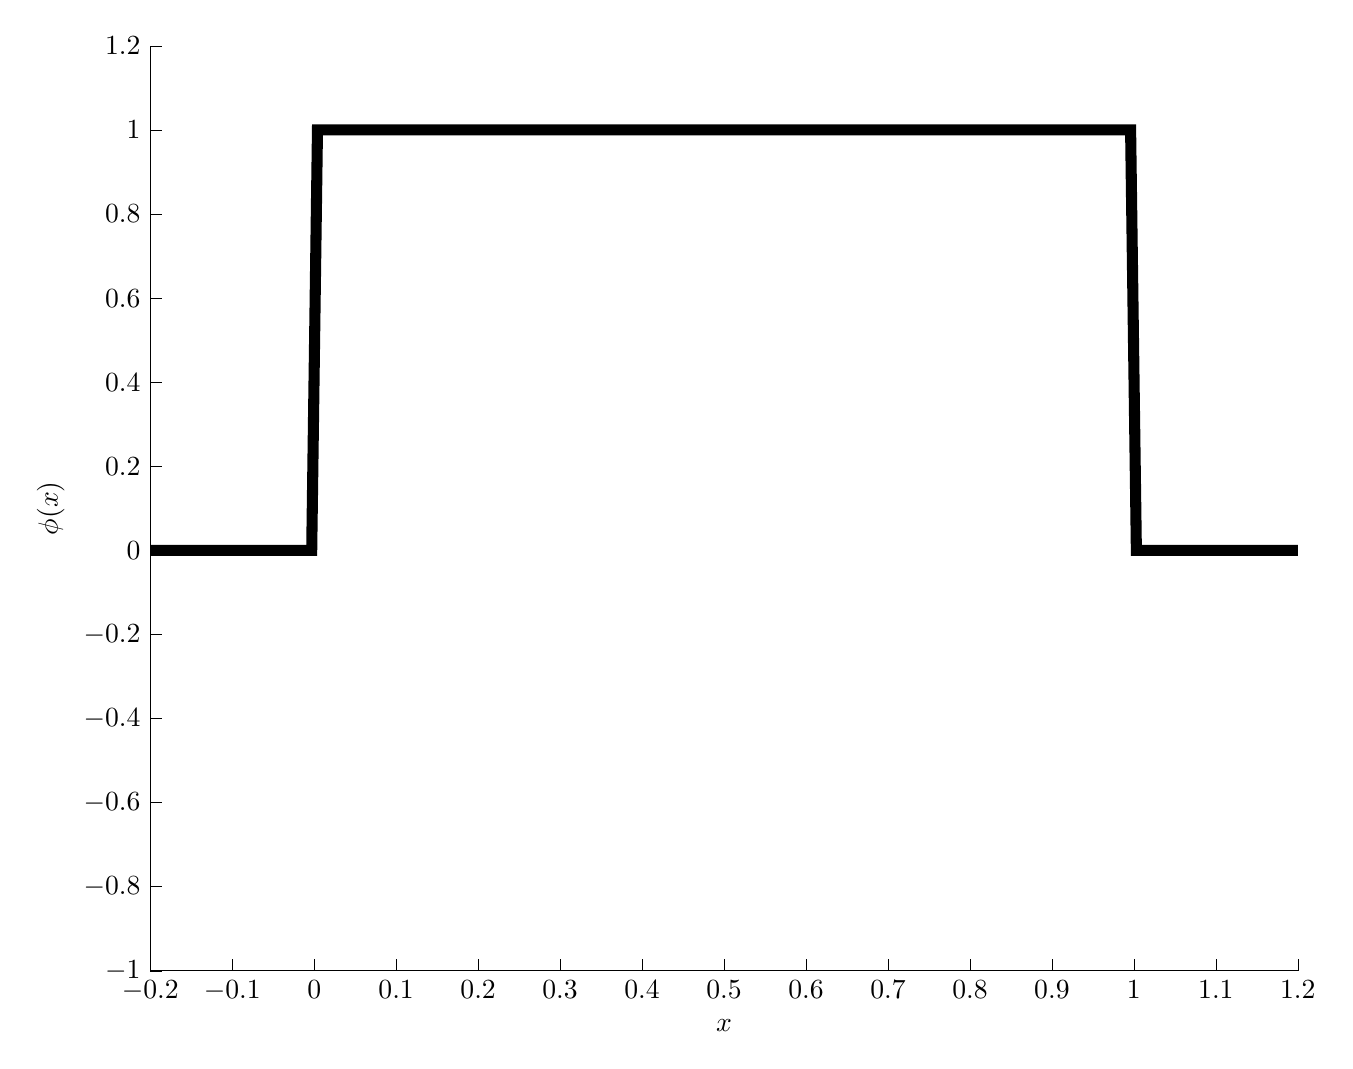
\begin{tikzpicture}

\begin{axis}[%
width=5.738in,
height=4.625in,
at={(1.29in,0.763in)},
scale only axis,
every outer x axis line/.append style={black},
every x tick label/.append style={font=\color{black}},
every x tick/.append style={black},
xmin=-0.2,
xmax=1.2,
xlabel={$x$},
every outer y axis line/.append style={black},
every y tick label/.append style={font=\color{black}},
every y tick/.append style={black},
ymin=-1,
ymax=1.2,
ylabel={$\phi(x)$},
axis background/.style={fill=white},
axis x line*=bottom,
axis y line*=left
]
\addplot [color=black, line width=4.0pt, forget plot]
  table[row sep=crcr]{%
-0.2	0\\
-0.192964824120603	0\\
-0.185929648241206	0\\
-0.178894472361809	0\\
-0.171859296482412	0\\
-0.164824120603015	0\\
-0.157788944723618	0\\
-0.150753768844221	0\\
-0.143718592964824	0\\
-0.136683417085427	0\\
-0.12964824120603	0\\
-0.122613065326633	0\\
-0.115577889447236	0\\
-0.108542713567839	0\\
-0.101507537688442	0\\
-0.0944723618090452	0\\
-0.0874371859296483	0\\
-0.0804020100502513	0\\
-0.0733668341708543	0\\
-0.0663316582914573	0\\
-0.0592964824120603	0\\
-0.0522613065326633	0\\
-0.0452261306532664	0\\
-0.0381909547738694	0\\
-0.0311557788944724	0\\
-0.0241206030150754	0\\
-0.0170854271356784	0\\
-0.0100502512562814	0\\
-0.00301507537688445	0\\
0.00402010050251253	1\\
0.0110552763819095	1\\
0.0180904522613065	1\\
0.0251256281407035	1\\
0.0321608040201005	1\\
0.0391959798994974	1\\
0.0462311557788945	1\\
0.0532663316582914	1\\
0.0603015075376884	1\\
0.0673366834170854	1\\
0.0743718592964824	1\\
0.0814070351758794	1\\
0.0884422110552764	1\\
0.0954773869346733	1\\
0.10251256281407	1\\
0.109547738693467	1\\
0.116582914572864	1\\
0.123618090452261	1\\
0.130653266331658	1\\
0.137688442211055	1\\
0.144723618090452	1\\
0.151758793969849	1\\
0.158793969849246	1\\
0.165829145728643	1\\
0.17286432160804	1\\
0.179899497487437	1\\
0.186934673366834	1\\
0.193969849246231	1\\
0.201005025125628	1\\
0.208040201005025	1\\
0.215075376884422	1\\
0.222110552763819	1\\
0.229145728643216	1\\
0.236180904522613	1\\
0.24321608040201	1\\
0.250251256281407	1\\
0.257286432160804	1\\
0.264321608040201	1\\
0.271356783919598	1\\
0.278391959798995	1\\
0.285427135678392	1\\
0.292462311557789	1\\
0.299497487437186	1\\
0.306532663316583	1\\
0.31356783919598	1\\
0.320603015075377	1\\
0.327638190954774	1\\
0.334673366834171	1\\
0.341708542713568	1\\
0.348743718592965	1\\
0.355778894472362	1\\
0.362814070351759	1\\
0.369849246231156	1\\
0.376884422110553	1\\
0.38391959798995	1\\
0.390954773869347	1\\
0.397989949748744	1\\
0.405025125628141	1\\
0.412060301507538	1\\
0.419095477386935	1\\
0.426130653266332	1\\
0.433165829145729	1\\
0.440201005025126	1\\
0.447236180904522	1\\
0.45427135678392	1\\
0.461306532663317	1\\
0.468341708542714	1\\
0.47537688442211	1\\
0.482412060301507	1\\
0.489447236180904	1\\
0.496482412060301	1\\
0.503517587939698	1\\
0.510552763819095	1\\
0.517587939698492	1\\
0.524623115577889	1\\
0.531658291457286	1\\
0.538693467336683	1\\
0.54572864321608	1\\
0.552763819095477	1\\
0.559798994974874	1\\
0.566834170854271	1\\
0.573869346733668	1\\
0.580904522613065	1\\
0.587939698492462	1\\
0.594974874371859	1\\
0.602010050251256	1\\
0.609045226130653	1\\
0.61608040201005	1\\
0.623115577889447	1\\
0.630150753768844	1\\
0.637185929648241	1\\
0.644221105527638	1\\
0.651256281407035	1\\
0.658291457286432	1\\
0.665326633165829	1\\
0.672361809045226	1\\
0.679396984924623	1\\
0.68643216080402	1\\
0.693467336683417	1\\
0.700502512562814	1\\
0.707537688442211	1\\
0.714572864321608	1\\
0.721608040201005	1\\
0.728643216080402	1\\
0.735678391959799	1\\
0.742713567839196	1\\
0.749748743718593	1\\
0.75678391959799	1\\
0.763819095477387	1\\
0.770854271356784	1\\
0.777889447236181	1\\
0.784924623115578	1\\
0.791959798994975	1\\
0.798994974874372	1\\
0.806030150753769	1\\
0.813065326633166	1\\
0.820100502512563	1\\
0.82713567839196	1\\
0.834170854271357	1\\
0.841206030150754	1\\
0.848241206030151	1\\
0.855276381909548	1\\
0.862311557788945	1\\
0.869346733668342	1\\
0.876381909547739	1\\
0.883417085427136	1\\
0.890452261306533	1\\
0.89748743718593	1\\
0.904522613065327	1\\
0.911557788944724	1\\
0.918592964824121	1\\
0.925628140703518	1\\
0.932663316582915	1\\
0.939698492462312	1\\
0.946733668341708	1\\
0.953768844221106	1\\
0.960804020100502	1\\
0.9678391959799	1\\
0.974874371859296	1\\
0.981909547738693	1\\
0.98894472361809	1\\
0.995979899497487	1\\
1.00301507537688	0\\
1.01005025125628	0\\
1.01708542713568	0\\
1.02412060301508	0\\
1.03115577889447	0\\
1.03819095477387	0\\
1.04522613065327	0\\
1.05226130653266	0\\
1.05929648241206	0\\
1.06633165829146	0\\
1.07336683417085	0\\
1.08040201005025	0\\
1.08743718592965	0\\
1.09447236180905	0\\
1.10150753768844	0\\
1.10854271356784	0\\
1.11557788944724	0\\
1.12261306532663	0\\
1.12964824120603	0\\
1.13668341708543	0\\
1.14371859296482	0\\
1.15075376884422	0\\
1.15778894472362	0\\
1.16482412060301	0\\
1.17185929648241	0\\
1.17889447236181	0\\
1.18592964824121	0\\
1.1929648241206	0\\
1.2	0\\
};
\end{axis}
\end{tikzpicture}%
	\caption{Haar scaling function}
	\label{fig:haar_scaling}
\end{figure}

\begin{figure}[H]
	\centering
	% GNUPLOT: LaTeX picture
\setlength{\unitlength}{0.240900pt}
\ifx\plotpoint\undefined\newsavebox{\plotpoint}\fi
\sbox{\plotpoint}{\rule[-0.200pt]{0.400pt}{0.400pt}}%
\begin{picture}(1500,900)(0,0)
\sbox{\plotpoint}{\rule[-0.200pt]{0.400pt}{0.400pt}}%
\put(171.0,192.0){\rule[-0.200pt]{4.818pt}{0.400pt}}
\put(151,192){\makebox(0,0)[r]{$-1$}}
\put(1419.0,192.0){\rule[-0.200pt]{4.818pt}{0.400pt}}
\put(171.0,343.0){\rule[-0.200pt]{4.818pt}{0.400pt}}
\put(151,343){\makebox(0,0)[r]{$-0.5$}}
\put(1419.0,343.0){\rule[-0.200pt]{4.818pt}{0.400pt}}
\put(171.0,495.0){\rule[-0.200pt]{4.818pt}{0.400pt}}
\put(151,495){\makebox(0,0)[r]{$0$}}
\put(1419.0,495.0){\rule[-0.200pt]{4.818pt}{0.400pt}}
\put(171.0,647.0){\rule[-0.200pt]{4.818pt}{0.400pt}}
\put(151,647){\makebox(0,0)[r]{$0.5$}}
\put(1419.0,647.0){\rule[-0.200pt]{4.818pt}{0.400pt}}
\put(171.0,798.0){\rule[-0.200pt]{4.818pt}{0.400pt}}
\put(151,798){\makebox(0,0)[r]{$1$}}
\put(1419.0,798.0){\rule[-0.200pt]{4.818pt}{0.400pt}}
\put(171.0,131.0){\rule[-0.200pt]{0.400pt}{4.818pt}}
\put(171,90){\makebox(0,0){$-0.2$}}
\put(171.0,839.0){\rule[-0.200pt]{0.400pt}{4.818pt}}
\put(352.0,131.0){\rule[-0.200pt]{0.400pt}{4.818pt}}
\put(352,90){\makebox(0,0){$0$}}
\put(352.0,839.0){\rule[-0.200pt]{0.400pt}{4.818pt}}
\put(533.0,131.0){\rule[-0.200pt]{0.400pt}{4.818pt}}
\put(533,90){\makebox(0,0){$0.2$}}
\put(533.0,839.0){\rule[-0.200pt]{0.400pt}{4.818pt}}
\put(714.0,131.0){\rule[-0.200pt]{0.400pt}{4.818pt}}
\put(714,90){\makebox(0,0){$0.4$}}
\put(714.0,839.0){\rule[-0.200pt]{0.400pt}{4.818pt}}
\put(896.0,131.0){\rule[-0.200pt]{0.400pt}{4.818pt}}
\put(896,90){\makebox(0,0){$0.6$}}
\put(896.0,839.0){\rule[-0.200pt]{0.400pt}{4.818pt}}
\put(1077.0,131.0){\rule[-0.200pt]{0.400pt}{4.818pt}}
\put(1077,90){\makebox(0,0){$0.8$}}
\put(1077.0,839.0){\rule[-0.200pt]{0.400pt}{4.818pt}}
\put(1258.0,131.0){\rule[-0.200pt]{0.400pt}{4.818pt}}
\put(1258,90){\makebox(0,0){$1$}}
\put(1258.0,839.0){\rule[-0.200pt]{0.400pt}{4.818pt}}
\put(1439.0,131.0){\rule[-0.200pt]{0.400pt}{4.818pt}}
\put(1439,90){\makebox(0,0){$1.2$}}
\put(1439.0,839.0){\rule[-0.200pt]{0.400pt}{4.818pt}}
\put(171.0,131.0){\rule[-0.200pt]{0.400pt}{175.375pt}}
\put(171.0,131.0){\rule[-0.200pt]{305.461pt}{0.400pt}}
\put(1439.0,131.0){\rule[-0.200pt]{0.400pt}{175.375pt}}
\put(171.0,859.0){\rule[-0.200pt]{305.461pt}{0.400pt}}
\put(30,495){\makebox(0,0){$\psi(x)$}}
\put(805,29){\makebox(0,0){$x$}}
\put(171,495){\usebox{\plotpoint}}
\multiput(349.59,495.00)(0.485,23.071){11}{\rule{0.117pt}{17.414pt}}
\multiput(348.17,495.00)(7.000,266.856){2}{\rule{0.400pt}{8.707pt}}
\put(171.0,495.0){\rule[-0.200pt]{42.880pt}{0.400pt}}
\multiput(802.59,629.88)(0.482,-54.735){9}{\rule{0.116pt}{40.500pt}}
\multiput(801.17,713.94)(6.000,-521.940){2}{\rule{0.400pt}{20.250pt}}
\put(356.0,798.0){\rule[-0.200pt]{107.441pt}{0.400pt}}
\multiput(1254.59,192.00)(0.485,23.071){11}{\rule{0.117pt}{17.414pt}}
\multiput(1253.17,192.00)(7.000,266.856){2}{\rule{0.400pt}{8.707pt}}
\put(808.0,192.0){\rule[-0.200pt]{107.441pt}{0.400pt}}
\put(1261.0,495.0){\rule[-0.200pt]{42.880pt}{0.400pt}}
\put(171.0,131.0){\rule[-0.200pt]{0.400pt}{175.375pt}}
\put(171.0,131.0){\rule[-0.200pt]{305.461pt}{0.400pt}}
\put(1439.0,131.0){\rule[-0.200pt]{0.400pt}{175.375pt}}
\put(171.0,859.0){\rule[-0.200pt]{305.461pt}{0.400pt}}
\end{picture}

	\caption{Haar wavelet function}
	\label{fig:haar_wavelet}
\end{figure}
Since the wavelet functions are localized in space, it is necessary to shift them in order to approximate
a function. This action is referred to as \textit{translation}. Furthermore, functions may exhibit very sharp changes over an
interval which is smaller than the piecewise constant wavelet, and so a wavelet of higher frequency is necessary
to fit the function. By using a \textit{dilation} of the original wavelet, the function can be well approximated. 
Define a relationship between the scaling function $\phi(x)$ and the translates of its dilation 
$\phi(2x)$ by the dilation equation given by
\begin{equation}
\phi(x) = \sum_{k=0}^{N} c_k \phi(2x-k).
\label{dilation equation}
\end{equation}

The three pillars(?) of wavelets which make them such a useful tool for approximation are \textbf{Orthogonality}, 
\textbf{Compact Support}, and \textbf{Multiresolution Analysis}.
\subsection{Orthogonality}
The basis of wavelet functions constitute an orthonormal set. All translations and dilations of the mother wavelet $\psi(x)$
are orthogonal to the scaling function $\phi(x)$, 
\begin{equation}
\int_{-\infty}^{\infty} \phi(x) \psi(x) dx = 0,
\end{equation}
and other wavelets
\begin{equation}
\int_{-\infty}^{\infty} \psi_{k}^{j}(x) \psi_{k'}^{j'}(x) dx = 0.
\end{equation}
\subsection{Compact Support}
Wavelet functions have compact support, implying that they are uniformly zero outside of a specified interval.
This property is advantageous for approximating sharp signals, where one would like to represent the spike using only a small 
handful of basis functions. The Fourier basis is not adequate for this purpose, since the support for the basis is global; 
the sine and cosine functions have infinite length. 
\subsection{Multiresolution Analysis}
Let us define the space which is spanned by the basis of scaling functions $\phi_{k}^{0}(x)$ at the coarsest
level of resolution by $V_0$. We understand from the previous section that the set of wavelet functions are orthogonal 
to the set of scaling functions, and so the space spanned by the basis of wavelet functions, denoted by $W_0$, is thusly
orthogonal to $V_0$. The refined space $V_1$ can be described by
\begin{equation}
V_1 = V_0 \oplus W_0,
\label{V1}
\end{equation}
which represents all piecewise functions defined on half-intervals. Equation (\ref{V1}) indicates that the space spanned by 
$\phi(2x)$ can be described by the `summation' of the spaces spanned by
$V_0$ and $W_0$. One finer level, $V_2$, is spanned by translates of $\phi(4x)$. It can be written as
\begin{equation}
V_2 = V_1 \oplus W_1 = V_0 \oplus W_0 \oplus W_1.
\label{V2}
\end{equation}
Considering successively finer approximation spaces spanned by $\phi(4x), \phi(8x), \dots, \phi(2^j x)$, yields the spaces
\begin{equation}
V_j = V_0 \oplus W_0 \oplus W_1 \oplus \dots \oplus W_j.
\end{equation}
The spaces $V_j$ are nested, since for example the function $\phi(x)$ is a combination of $\phi(2x)$ and $\phi(2x-1)$. 
In other terms, $V_0 \subset V_1 \subset \dots \subset V_j$.
\subsection{Dyadic Grid}
The multi-resolution properties of wavelets previously described warrant a multilevel, or dyadic grid.
This grid should have as many levels as there are scales in the given problem. It can consist of 
either uniformly or non-uniformly spaced points. In the case of equally spaced grid points, 
let each grid level $j = 0, \dots, J$ be computed by 
\begin{align}
x^{j}_{k} &= 2^{-(j+\delta)} k,\text{ } \text{ } \text{ }  \text{ for $k=0,\dots,2^{j+\delta}$ },
\end{align}
where $\delta$ is some integer shifting parameter, allowing one to dictate that the coarsest level of resolution have 
smaller spacing than $1$ as in the case where $\delta=0$. From here forth we keep omit the parameter $\delta$, but keep
in mind that the number of grid points at each level may be shifted at will based on a fixed choice of $\delta$. 
The grid levels are formally defined by 
\begin{equation}
    \mathcal{G}^j= \{ x_{k}^{j} \in \Omega : k \in \mathcal{K}^j \}, \text{ } j \in \mathcal{Z},
\end{equation}
where $\mathcal{K}^{j}$ is the integer set representing the spatial locations in the grid at level $j$. The grids are 
nested, implying that $\mathcal{G}^{j} \subset \mathcal{G}^{j+1}$. In other words, the points $x^{j}$ are a perfect 
subset of the points $x^{j+1}$. This can be demonstrated by the relation that 
$x_{k}^{j}=x_{2k}^{j+1}$ for $k \in \mathcal{K}^{j}$.

\section{Second-Generation Wavelets}
Second-generation wavelets refer to the family of functions which are no longer defined as translates and dilations of 
a single mother function. 

\subsection{Interpolating Subdivision}
The interpolating subdivision scheme is central to the second-generation wavelet collocation approach. The scheme is used to
approximate values at odd points $x_{2k+1}^{j+1}$ by using $2N$ nearest points to construct interpolating polynomials of 
order $2N-1$. Lagrange polynomials are used, and the method can be used with a uniform grid or with 
nonuniform points such as Chebyshev points. The interpolating scheme is 
\begin{equation}
    f(x_{2k+1}^{j+1})=\sum_{l=-N+1}^{N} L_{k+l} f(x_{k+l}^{j}), \label{interp}
\end{equation}
where the interpolating weights are Lagrange polynomial coefficients given by 
\begin{equation}
    L_{k+l}(x)=\prod_{ \substack{ i=k-N+1 \\ i\neq k+l } }^{k+N} \frac{x-x_i}{x_{k+l}-x_i}.
\end{equation}
Given a uniform grid spacing at level $j$ of $h^j$, the accuracy of such an interpolation is of $\mathcal{O}((h^{j})^{2N})$.  

\subsection{Wavelet Transform}
The existence of a fast wavelet transform is one of the attractive qualities of the method. The transform makes use of the 
interpolating subdivision algorithm (\ref{interp}) for the calculation of the scaling and detail wavelet coefficients. The forward wavelet transform is given by
\begin{equation}
	\begin{split}
		d_{k}^{j} &= \frac{1}{2} \left( c_{2k+1}^{j+1}-\sum_{l} w_{k,l}^{j} c_{2k+2l}^{j+1} \right), \\
		c_{k}^{j} &= c_{2k}^{j+1},
	\end{split}
\end{equation}
and the inverse transform is given by 
\begin{equation}
	\begin{split}
		c_{2k+1}^{j+1} &= 2 d_{k}^{j}  + \sum_{l} w_{k,l}^{j} c_{k+l}^{j}, \\
		c_{2k}^{j+1} &= c_{k}^{j}.
	\end{split}
\end{equation}

\subsection{Construction of Interpolating Scaling and Wavelet Functions}
The wavelet and scaling function do not have a closed-form expression.
\subsubsection{Scaling Functions}
The construction of second-generation interpolating wavelets makes use of the interpolating subdivision algorithm. 
The scheme is used to interpolate functional values defined at points on level $j$, to odd points (i.e. $x_{2k+1}^{j+1}$) 
at the next higher level of resolution. This scheme is used to construct the scaling and detail wavelet functions. 
Examples of the scaling and detail functions are shown in Figure 1 and Figure 2 respectively.
To obtain the scaling function $\phi_{m}^{j}(x)$, from (5) set $c_{k}^{j}=\delta_{k,m}, \forall k \in \mathcal{K}^j$, where $\delta_{k,m}$ is the Kronecker delta function defined by
\[ \delta_{k,m} = \begin{cases} 
      1 & k=m \\
      0 & k \neq m.
   \end{cases}
\]
Then let all $d_{l}^{j'}=0, \forall l \in \mathcal{L}^{j'}, \forall j' \geq j$ and perform the inverse transform up to an arbitrarily high level of resolution $J$. 

\subsubsection{Wavelet Functions}
The wavelet $\psi_{l}^{j}$ is computed by setting $d_{m}^{j'} = \delta_{j',j} \delta_{l,m}, \forall l \in \mathcal{L}^{j}, \forall j \geq j$, and also $c_{k}^{j}, \forall k \in \mathcal{K}^j$. Then perform the inverse wavelet transform up to an arbitrarily high level of resolution $J$.

\begin{figure}
	\center
	% GNUPLOT: LaTeX picture
\setlength{\unitlength}{0.240900pt}
\ifx\plotpoint\undefined\newsavebox{\plotpoint}\fi
\sbox{\plotpoint}{\rule[-0.200pt]{0.400pt}{0.400pt}}%
\begin{picture}(1500,900)(0,0)
\sbox{\plotpoint}{\rule[-0.200pt]{0.400pt}{0.400pt}}%
\put(171.0,131.0){\rule[-0.200pt]{4.818pt}{0.400pt}}
\put(151,131){\makebox(0,0)[r]{$-0.2$}}
\put(1419.0,131.0){\rule[-0.200pt]{4.818pt}{0.400pt}}
\put(171.0,252.0){\rule[-0.200pt]{4.818pt}{0.400pt}}
\put(151,252){\makebox(0,0)[r]{$0$}}
\put(1419.0,252.0){\rule[-0.200pt]{4.818pt}{0.400pt}}
\put(171.0,374.0){\rule[-0.200pt]{4.818pt}{0.400pt}}
\put(151,374){\makebox(0,0)[r]{$0.2$}}
\put(1419.0,374.0){\rule[-0.200pt]{4.818pt}{0.400pt}}
\put(171.0,495.0){\rule[-0.200pt]{4.818pt}{0.400pt}}
\put(151,495){\makebox(0,0)[r]{$0.4$}}
\put(1419.0,495.0){\rule[-0.200pt]{4.818pt}{0.400pt}}
\put(171.0,616.0){\rule[-0.200pt]{4.818pt}{0.400pt}}
\put(151,616){\makebox(0,0)[r]{$0.6$}}
\put(1419.0,616.0){\rule[-0.200pt]{4.818pt}{0.400pt}}
\put(171.0,738.0){\rule[-0.200pt]{4.818pt}{0.400pt}}
\put(151,738){\makebox(0,0)[r]{$0.8$}}
\put(1419.0,738.0){\rule[-0.200pt]{4.818pt}{0.400pt}}
\put(171.0,859.0){\rule[-0.200pt]{4.818pt}{0.400pt}}
\put(151,859){\makebox(0,0)[r]{$1$}}
\put(1419.0,859.0){\rule[-0.200pt]{4.818pt}{0.400pt}}
\put(171.0,131.0){\rule[-0.200pt]{0.400pt}{4.818pt}}
\put(171,90){\makebox(0,0){$-4$}}
\put(171.0,839.0){\rule[-0.200pt]{0.400pt}{4.818pt}}
\put(330.0,131.0){\rule[-0.200pt]{0.400pt}{4.818pt}}
\put(330,90){\makebox(0,0){$-3$}}
\put(330.0,839.0){\rule[-0.200pt]{0.400pt}{4.818pt}}
\put(488.0,131.0){\rule[-0.200pt]{0.400pt}{4.818pt}}
\put(488,90){\makebox(0,0){$-2$}}
\put(488.0,839.0){\rule[-0.200pt]{0.400pt}{4.818pt}}
\put(647.0,131.0){\rule[-0.200pt]{0.400pt}{4.818pt}}
\put(647,90){\makebox(0,0){$-1$}}
\put(647.0,839.0){\rule[-0.200pt]{0.400pt}{4.818pt}}
\put(805.0,131.0){\rule[-0.200pt]{0.400pt}{4.818pt}}
\put(805,90){\makebox(0,0){$0$}}
\put(805.0,839.0){\rule[-0.200pt]{0.400pt}{4.818pt}}
\put(964.0,131.0){\rule[-0.200pt]{0.400pt}{4.818pt}}
\put(964,90){\makebox(0,0){$1$}}
\put(964.0,839.0){\rule[-0.200pt]{0.400pt}{4.818pt}}
\put(1122.0,131.0){\rule[-0.200pt]{0.400pt}{4.818pt}}
\put(1122,90){\makebox(0,0){$2$}}
\put(1122.0,839.0){\rule[-0.200pt]{0.400pt}{4.818pt}}
\put(1281.0,131.0){\rule[-0.200pt]{0.400pt}{4.818pt}}
\put(1281,90){\makebox(0,0){$3$}}
\put(1281.0,839.0){\rule[-0.200pt]{0.400pt}{4.818pt}}
\put(1439.0,131.0){\rule[-0.200pt]{0.400pt}{4.818pt}}
\put(1439,90){\makebox(0,0){$4$}}
\put(1439.0,839.0){\rule[-0.200pt]{0.400pt}{4.818pt}}
\put(171.0,131.0){\rule[-0.200pt]{0.400pt}{175.375pt}}
\put(171.0,131.0){\rule[-0.200pt]{305.461pt}{0.400pt}}
\put(1439.0,131.0){\rule[-0.200pt]{0.400pt}{175.375pt}}
\put(171.0,859.0){\rule[-0.200pt]{305.461pt}{0.400pt}}
\put(30,495){\makebox(0,0){$\phi(x)$}}
\put(805,29){\makebox(0,0){$x$}}
\put(171,252){\usebox{\plotpoint}}
\put(567,251.67){\rule{1.204pt}{0.400pt}}
\multiput(567.00,251.17)(2.500,1.000){2}{\rule{0.602pt}{0.400pt}}
\put(572,252.67){\rule{1.204pt}{0.400pt}}
\multiput(572.00,252.17)(2.500,1.000){2}{\rule{0.602pt}{0.400pt}}
\put(577,253.67){\rule{1.204pt}{0.400pt}}
\multiput(577.00,253.17)(2.500,1.000){2}{\rule{0.602pt}{0.400pt}}
\put(582,254.67){\rule{1.204pt}{0.400pt}}
\multiput(582.00,254.17)(2.500,1.000){2}{\rule{0.602pt}{0.400pt}}
\put(587,255.67){\rule{1.204pt}{0.400pt}}
\multiput(587.00,255.17)(2.500,1.000){2}{\rule{0.602pt}{0.400pt}}
\put(592,256.67){\rule{1.204pt}{0.400pt}}
\multiput(592.00,256.17)(2.500,1.000){2}{\rule{0.602pt}{0.400pt}}
\put(171.0,252.0){\rule[-0.200pt]{95.396pt}{0.400pt}}
\put(602,257.67){\rule{1.204pt}{0.400pt}}
\multiput(602.00,257.17)(2.500,1.000){2}{\rule{0.602pt}{0.400pt}}
\put(607,259.17){\rule{1.100pt}{0.400pt}}
\multiput(607.00,258.17)(2.717,2.000){2}{\rule{0.550pt}{0.400pt}}
\put(612,260.67){\rule{1.204pt}{0.400pt}}
\multiput(612.00,260.17)(2.500,1.000){2}{\rule{0.602pt}{0.400pt}}
\put(597.0,258.0){\rule[-0.200pt]{1.204pt}{0.400pt}}
\put(632,260.17){\rule{1.100pt}{0.400pt}}
\multiput(632.00,261.17)(2.717,-2.000){2}{\rule{0.550pt}{0.400pt}}
\multiput(637.00,258.95)(0.909,-0.447){3}{\rule{0.767pt}{0.108pt}}
\multiput(637.00,259.17)(3.409,-3.000){2}{\rule{0.383pt}{0.400pt}}
\multiput(642.00,255.93)(0.487,-0.477){7}{\rule{0.500pt}{0.115pt}}
\multiput(642.00,256.17)(3.962,-5.000){2}{\rule{0.250pt}{0.400pt}}
\multiput(647.60,249.09)(0.468,-0.774){5}{\rule{0.113pt}{0.700pt}}
\multiput(646.17,250.55)(4.000,-4.547){2}{\rule{0.400pt}{0.350pt}}
\multiput(651.59,242.93)(0.477,-0.821){7}{\rule{0.115pt}{0.740pt}}
\multiput(650.17,244.46)(5.000,-6.464){2}{\rule{0.400pt}{0.370pt}}
\multiput(656.59,234.93)(0.477,-0.821){7}{\rule{0.115pt}{0.740pt}}
\multiput(655.17,236.46)(5.000,-6.464){2}{\rule{0.400pt}{0.370pt}}
\multiput(661.59,226.60)(0.477,-0.933){7}{\rule{0.115pt}{0.820pt}}
\multiput(660.17,228.30)(5.000,-7.298){2}{\rule{0.400pt}{0.410pt}}
\multiput(666.59,217.93)(0.477,-0.821){7}{\rule{0.115pt}{0.740pt}}
\multiput(665.17,219.46)(5.000,-6.464){2}{\rule{0.400pt}{0.370pt}}
\multiput(671.59,210.26)(0.477,-0.710){7}{\rule{0.115pt}{0.660pt}}
\multiput(670.17,211.63)(5.000,-5.630){2}{\rule{0.400pt}{0.330pt}}
\multiput(676.59,203.26)(0.477,-0.710){7}{\rule{0.115pt}{0.660pt}}
\multiput(675.17,204.63)(5.000,-5.630){2}{\rule{0.400pt}{0.330pt}}
\multiput(681.59,196.59)(0.477,-0.599){7}{\rule{0.115pt}{0.580pt}}
\multiput(680.17,197.80)(5.000,-4.796){2}{\rule{0.400pt}{0.290pt}}
\multiput(686.00,191.94)(0.627,-0.468){5}{\rule{0.600pt}{0.113pt}}
\multiput(686.00,192.17)(3.755,-4.000){2}{\rule{0.300pt}{0.400pt}}
\multiput(691.00,187.95)(0.909,-0.447){3}{\rule{0.767pt}{0.108pt}}
\multiput(691.00,188.17)(3.409,-3.000){2}{\rule{0.383pt}{0.400pt}}
\put(617.0,262.0){\rule[-0.200pt]{3.613pt}{0.400pt}}
\multiput(701.00,186.60)(0.627,0.468){5}{\rule{0.600pt}{0.113pt}}
\multiput(701.00,185.17)(3.755,4.000){2}{\rule{0.300pt}{0.400pt}}
\multiput(706.59,190.00)(0.477,0.821){7}{\rule{0.115pt}{0.740pt}}
\multiput(705.17,190.00)(5.000,6.464){2}{\rule{0.400pt}{0.370pt}}
\multiput(711.59,198.00)(0.477,1.267){7}{\rule{0.115pt}{1.060pt}}
\multiput(710.17,198.00)(5.000,9.800){2}{\rule{0.400pt}{0.530pt}}
\multiput(716.59,210.00)(0.477,1.935){7}{\rule{0.115pt}{1.540pt}}
\multiput(715.17,210.00)(5.000,14.804){2}{\rule{0.400pt}{0.770pt}}
\multiput(721.59,228.00)(0.477,2.602){7}{\rule{0.115pt}{2.020pt}}
\multiput(720.17,228.00)(5.000,19.807){2}{\rule{0.400pt}{1.010pt}}
\multiput(726.59,252.00)(0.477,3.493){7}{\rule{0.115pt}{2.660pt}}
\multiput(725.17,252.00)(5.000,26.479){2}{\rule{0.400pt}{1.330pt}}
\multiput(731.59,284.00)(0.477,4.161){7}{\rule{0.115pt}{3.140pt}}
\multiput(730.17,284.00)(5.000,31.483){2}{\rule{0.400pt}{1.570pt}}
\multiput(736.59,322.00)(0.477,4.718){7}{\rule{0.115pt}{3.540pt}}
\multiput(735.17,322.00)(5.000,35.653){2}{\rule{0.400pt}{1.770pt}}
\multiput(741.59,365.00)(0.477,5.051){7}{\rule{0.115pt}{3.780pt}}
\multiput(740.17,365.00)(5.000,38.154){2}{\rule{0.400pt}{1.890pt}}
\multiput(746.59,411.00)(0.477,5.274){7}{\rule{0.115pt}{3.940pt}}
\multiput(745.17,411.00)(5.000,39.822){2}{\rule{0.400pt}{1.970pt}}
\multiput(751.60,459.00)(0.468,7.207){5}{\rule{0.113pt}{5.100pt}}
\multiput(750.17,459.00)(4.000,39.415){2}{\rule{0.400pt}{2.550pt}}
\multiput(755.59,509.00)(0.477,5.385){7}{\rule{0.115pt}{4.020pt}}
\multiput(754.17,509.00)(5.000,40.656){2}{\rule{0.400pt}{2.010pt}}
\multiput(760.59,558.00)(0.477,5.497){7}{\rule{0.115pt}{4.100pt}}
\multiput(759.17,558.00)(5.000,41.490){2}{\rule{0.400pt}{2.050pt}}
\multiput(765.59,608.00)(0.477,5.274){7}{\rule{0.115pt}{3.940pt}}
\multiput(764.17,608.00)(5.000,39.822){2}{\rule{0.400pt}{1.970pt}}
\multiput(770.59,656.00)(0.477,5.051){7}{\rule{0.115pt}{3.780pt}}
\multiput(769.17,656.00)(5.000,38.154){2}{\rule{0.400pt}{1.890pt}}
\multiput(775.59,702.00)(0.477,4.495){7}{\rule{0.115pt}{3.380pt}}
\multiput(774.17,702.00)(5.000,33.985){2}{\rule{0.400pt}{1.690pt}}
\multiput(780.59,743.00)(0.477,4.161){7}{\rule{0.115pt}{3.140pt}}
\multiput(779.17,743.00)(5.000,31.483){2}{\rule{0.400pt}{1.570pt}}
\multiput(785.59,781.00)(0.477,3.382){7}{\rule{0.115pt}{2.580pt}}
\multiput(784.17,781.00)(5.000,25.645){2}{\rule{0.400pt}{1.290pt}}
\multiput(790.59,812.00)(0.477,2.714){7}{\rule{0.115pt}{2.100pt}}
\multiput(789.17,812.00)(5.000,20.641){2}{\rule{0.400pt}{1.050pt}}
\multiput(795.59,837.00)(0.477,1.712){7}{\rule{0.115pt}{1.380pt}}
\multiput(794.17,837.00)(5.000,13.136){2}{\rule{0.400pt}{0.690pt}}
\multiput(800.59,853.00)(0.477,0.599){7}{\rule{0.115pt}{0.580pt}}
\multiput(799.17,853.00)(5.000,4.796){2}{\rule{0.400pt}{0.290pt}}
\multiput(805.59,856.59)(0.477,-0.599){7}{\rule{0.115pt}{0.580pt}}
\multiput(804.17,857.80)(5.000,-4.796){2}{\rule{0.400pt}{0.290pt}}
\multiput(810.59,847.27)(0.477,-1.712){7}{\rule{0.115pt}{1.380pt}}
\multiput(809.17,850.14)(5.000,-13.136){2}{\rule{0.400pt}{0.690pt}}
\multiput(815.59,828.28)(0.477,-2.714){7}{\rule{0.115pt}{2.100pt}}
\multiput(814.17,832.64)(5.000,-20.641){2}{\rule{0.400pt}{1.050pt}}
\multiput(820.59,801.29)(0.477,-3.382){7}{\rule{0.115pt}{2.580pt}}
\multiput(819.17,806.65)(5.000,-25.645){2}{\rule{0.400pt}{1.290pt}}
\multiput(825.59,767.97)(0.477,-4.161){7}{\rule{0.115pt}{3.140pt}}
\multiput(824.17,774.48)(5.000,-31.483){2}{\rule{0.400pt}{1.570pt}}
\multiput(830.59,728.97)(0.477,-4.495){7}{\rule{0.115pt}{3.380pt}}
\multiput(829.17,735.98)(5.000,-33.985){2}{\rule{0.400pt}{1.690pt}}
\multiput(835.59,686.31)(0.477,-5.051){7}{\rule{0.115pt}{3.780pt}}
\multiput(834.17,694.15)(5.000,-38.154){2}{\rule{0.400pt}{1.890pt}}
\multiput(840.59,639.64)(0.477,-5.274){7}{\rule{0.115pt}{3.940pt}}
\multiput(839.17,647.82)(5.000,-39.822){2}{\rule{0.400pt}{1.970pt}}
\multiput(845.59,590.98)(0.477,-5.497){7}{\rule{0.115pt}{4.100pt}}
\multiput(844.17,599.49)(5.000,-41.490){2}{\rule{0.400pt}{2.050pt}}
\multiput(850.59,541.31)(0.477,-5.385){7}{\rule{0.115pt}{4.020pt}}
\multiput(849.17,549.66)(5.000,-40.656){2}{\rule{0.400pt}{2.010pt}}
\multiput(855.60,487.83)(0.468,-7.207){5}{\rule{0.113pt}{5.100pt}}
\multiput(854.17,498.41)(4.000,-39.415){2}{\rule{0.400pt}{2.550pt}}
\multiput(859.59,442.64)(0.477,-5.274){7}{\rule{0.115pt}{3.940pt}}
\multiput(858.17,450.82)(5.000,-39.822){2}{\rule{0.400pt}{1.970pt}}
\multiput(864.59,395.31)(0.477,-5.051){7}{\rule{0.115pt}{3.780pt}}
\multiput(863.17,403.15)(5.000,-38.154){2}{\rule{0.400pt}{1.890pt}}
\multiput(869.59,350.31)(0.477,-4.718){7}{\rule{0.115pt}{3.540pt}}
\multiput(868.17,357.65)(5.000,-35.653){2}{\rule{0.400pt}{1.770pt}}
\multiput(874.59,308.97)(0.477,-4.161){7}{\rule{0.115pt}{3.140pt}}
\multiput(873.17,315.48)(5.000,-31.483){2}{\rule{0.400pt}{1.570pt}}
\multiput(879.59,272.96)(0.477,-3.493){7}{\rule{0.115pt}{2.660pt}}
\multiput(878.17,278.48)(5.000,-26.479){2}{\rule{0.400pt}{1.330pt}}
\multiput(884.59,243.61)(0.477,-2.602){7}{\rule{0.115pt}{2.020pt}}
\multiput(883.17,247.81)(5.000,-19.807){2}{\rule{0.400pt}{1.010pt}}
\multiput(889.59,221.61)(0.477,-1.935){7}{\rule{0.115pt}{1.540pt}}
\multiput(888.17,224.80)(5.000,-14.804){2}{\rule{0.400pt}{0.770pt}}
\multiput(894.59,205.60)(0.477,-1.267){7}{\rule{0.115pt}{1.060pt}}
\multiput(893.17,207.80)(5.000,-9.800){2}{\rule{0.400pt}{0.530pt}}
\multiput(899.59,194.93)(0.477,-0.821){7}{\rule{0.115pt}{0.740pt}}
\multiput(898.17,196.46)(5.000,-6.464){2}{\rule{0.400pt}{0.370pt}}
\multiput(904.00,188.94)(0.627,-0.468){5}{\rule{0.600pt}{0.113pt}}
\multiput(904.00,189.17)(3.755,-4.000){2}{\rule{0.300pt}{0.400pt}}
\put(696.0,186.0){\rule[-0.200pt]{1.204pt}{0.400pt}}
\multiput(914.00,186.61)(0.909,0.447){3}{\rule{0.767pt}{0.108pt}}
\multiput(914.00,185.17)(3.409,3.000){2}{\rule{0.383pt}{0.400pt}}
\multiput(919.00,189.60)(0.627,0.468){5}{\rule{0.600pt}{0.113pt}}
\multiput(919.00,188.17)(3.755,4.000){2}{\rule{0.300pt}{0.400pt}}
\multiput(924.59,193.00)(0.477,0.599){7}{\rule{0.115pt}{0.580pt}}
\multiput(923.17,193.00)(5.000,4.796){2}{\rule{0.400pt}{0.290pt}}
\multiput(929.59,199.00)(0.477,0.710){7}{\rule{0.115pt}{0.660pt}}
\multiput(928.17,199.00)(5.000,5.630){2}{\rule{0.400pt}{0.330pt}}
\multiput(934.59,206.00)(0.477,0.710){7}{\rule{0.115pt}{0.660pt}}
\multiput(933.17,206.00)(5.000,5.630){2}{\rule{0.400pt}{0.330pt}}
\multiput(939.59,213.00)(0.477,0.821){7}{\rule{0.115pt}{0.740pt}}
\multiput(938.17,213.00)(5.000,6.464){2}{\rule{0.400pt}{0.370pt}}
\multiput(944.59,221.00)(0.477,0.933){7}{\rule{0.115pt}{0.820pt}}
\multiput(943.17,221.00)(5.000,7.298){2}{\rule{0.400pt}{0.410pt}}
\multiput(949.59,230.00)(0.477,0.821){7}{\rule{0.115pt}{0.740pt}}
\multiput(948.17,230.00)(5.000,6.464){2}{\rule{0.400pt}{0.370pt}}
\multiput(954.59,238.00)(0.477,0.821){7}{\rule{0.115pt}{0.740pt}}
\multiput(953.17,238.00)(5.000,6.464){2}{\rule{0.400pt}{0.370pt}}
\multiput(959.59,246.00)(0.477,0.599){7}{\rule{0.115pt}{0.580pt}}
\multiput(958.17,246.00)(5.000,4.796){2}{\rule{0.400pt}{0.290pt}}
\multiput(964.60,252.00)(0.468,0.627){5}{\rule{0.113pt}{0.600pt}}
\multiput(963.17,252.00)(4.000,3.755){2}{\rule{0.400pt}{0.300pt}}
\multiput(968.00,257.61)(0.909,0.447){3}{\rule{0.767pt}{0.108pt}}
\multiput(968.00,256.17)(3.409,3.000){2}{\rule{0.383pt}{0.400pt}}
\put(973,260.17){\rule{1.100pt}{0.400pt}}
\multiput(973.00,259.17)(2.717,2.000){2}{\rule{0.550pt}{0.400pt}}
\put(909.0,186.0){\rule[-0.200pt]{1.204pt}{0.400pt}}
\put(993,260.67){\rule{1.204pt}{0.400pt}}
\multiput(993.00,261.17)(2.500,-1.000){2}{\rule{0.602pt}{0.400pt}}
\put(998,259.17){\rule{1.100pt}{0.400pt}}
\multiput(998.00,260.17)(2.717,-2.000){2}{\rule{0.550pt}{0.400pt}}
\put(1003,257.67){\rule{1.204pt}{0.400pt}}
\multiput(1003.00,258.17)(2.500,-1.000){2}{\rule{0.602pt}{0.400pt}}
\put(978.0,262.0){\rule[-0.200pt]{3.613pt}{0.400pt}}
\put(1013,256.67){\rule{1.204pt}{0.400pt}}
\multiput(1013.00,257.17)(2.500,-1.000){2}{\rule{0.602pt}{0.400pt}}
\put(1018,255.67){\rule{1.204pt}{0.400pt}}
\multiput(1018.00,256.17)(2.500,-1.000){2}{\rule{0.602pt}{0.400pt}}
\put(1023,254.67){\rule{1.204pt}{0.400pt}}
\multiput(1023.00,255.17)(2.500,-1.000){2}{\rule{0.602pt}{0.400pt}}
\put(1028,253.67){\rule{1.204pt}{0.400pt}}
\multiput(1028.00,254.17)(2.500,-1.000){2}{\rule{0.602pt}{0.400pt}}
\put(1033,252.67){\rule{1.204pt}{0.400pt}}
\multiput(1033.00,253.17)(2.500,-1.000){2}{\rule{0.602pt}{0.400pt}}
\put(1038,251.67){\rule{1.204pt}{0.400pt}}
\multiput(1038.00,252.17)(2.500,-1.000){2}{\rule{0.602pt}{0.400pt}}
\put(1008.0,258.0){\rule[-0.200pt]{1.204pt}{0.400pt}}
\put(1043.0,252.0){\rule[-0.200pt]{95.396pt}{0.400pt}}
\put(171.0,131.0){\rule[-0.200pt]{0.400pt}{175.375pt}}
\put(171.0,131.0){\rule[-0.200pt]{305.461pt}{0.400pt}}
\put(1439.0,131.0){\rule[-0.200pt]{0.400pt}{175.375pt}}
\put(171.0,859.0){\rule[-0.200pt]{305.461pt}{0.400pt}}
\end{picture}

	\caption{An example of a scaling function, $\phi(x)$, for $N=3$.}
\end{figure}
\begin{figure}
	\center
	% GNUPLOT: LaTeX picture
\setlength{\unitlength}{0.240900pt}
\ifx\plotpoint\undefined\newsavebox{\plotpoint}\fi
\sbox{\plotpoint}{\rule[-0.200pt]{0.400pt}{0.400pt}}%
\begin{picture}(1500,900)(0,0)
\sbox{\plotpoint}{\rule[-0.200pt]{0.400pt}{0.400pt}}%
\put(171.0,131.0){\rule[-0.200pt]{4.818pt}{0.400pt}}
\put(151,131){\makebox(0,0)[r]{$-0.5$}}
\put(1419.0,131.0){\rule[-0.200pt]{4.818pt}{0.400pt}}
\put(171.0,277.0){\rule[-0.200pt]{4.818pt}{0.400pt}}
\put(151,277){\makebox(0,0)[r]{$0$}}
\put(1419.0,277.0){\rule[-0.200pt]{4.818pt}{0.400pt}}
\put(171.0,422.0){\rule[-0.200pt]{4.818pt}{0.400pt}}
\put(151,422){\makebox(0,0)[r]{$0.5$}}
\put(1419.0,422.0){\rule[-0.200pt]{4.818pt}{0.400pt}}
\put(171.0,568.0){\rule[-0.200pt]{4.818pt}{0.400pt}}
\put(151,568){\makebox(0,0)[r]{$1$}}
\put(1419.0,568.0){\rule[-0.200pt]{4.818pt}{0.400pt}}
\put(171.0,713.0){\rule[-0.200pt]{4.818pt}{0.400pt}}
\put(151,713){\makebox(0,0)[r]{$1.5$}}
\put(1419.0,713.0){\rule[-0.200pt]{4.818pt}{0.400pt}}
\put(171.0,859.0){\rule[-0.200pt]{4.818pt}{0.400pt}}
\put(151,859){\makebox(0,0)[r]{$2$}}
\put(1419.0,859.0){\rule[-0.200pt]{4.818pt}{0.400pt}}
\put(171.0,131.0){\rule[-0.200pt]{0.400pt}{4.818pt}}
\put(171,90){\makebox(0,0){$-4$}}
\put(171.0,839.0){\rule[-0.200pt]{0.400pt}{4.818pt}}
\put(330.0,131.0){\rule[-0.200pt]{0.400pt}{4.818pt}}
\put(330,90){\makebox(0,0){$-3$}}
\put(330.0,839.0){\rule[-0.200pt]{0.400pt}{4.818pt}}
\put(488.0,131.0){\rule[-0.200pt]{0.400pt}{4.818pt}}
\put(488,90){\makebox(0,0){$-2$}}
\put(488.0,839.0){\rule[-0.200pt]{0.400pt}{4.818pt}}
\put(647.0,131.0){\rule[-0.200pt]{0.400pt}{4.818pt}}
\put(647,90){\makebox(0,0){$-1$}}
\put(647.0,839.0){\rule[-0.200pt]{0.400pt}{4.818pt}}
\put(805.0,131.0){\rule[-0.200pt]{0.400pt}{4.818pt}}
\put(805,90){\makebox(0,0){$0$}}
\put(805.0,839.0){\rule[-0.200pt]{0.400pt}{4.818pt}}
\put(964.0,131.0){\rule[-0.200pt]{0.400pt}{4.818pt}}
\put(964,90){\makebox(0,0){$1$}}
\put(964.0,839.0){\rule[-0.200pt]{0.400pt}{4.818pt}}
\put(1122.0,131.0){\rule[-0.200pt]{0.400pt}{4.818pt}}
\put(1122,90){\makebox(0,0){$2$}}
\put(1122.0,839.0){\rule[-0.200pt]{0.400pt}{4.818pt}}
\put(1281.0,131.0){\rule[-0.200pt]{0.400pt}{4.818pt}}
\put(1281,90){\makebox(0,0){$3$}}
\put(1281.0,839.0){\rule[-0.200pt]{0.400pt}{4.818pt}}
\put(1439.0,131.0){\rule[-0.200pt]{0.400pt}{4.818pt}}
\put(1439,90){\makebox(0,0){$4$}}
\put(1439.0,839.0){\rule[-0.200pt]{0.400pt}{4.818pt}}
\put(171.0,131.0){\rule[-0.200pt]{0.400pt}{175.375pt}}
\put(171.0,131.0){\rule[-0.200pt]{305.461pt}{0.400pt}}
\put(1439.0,131.0){\rule[-0.200pt]{0.400pt}{175.375pt}}
\put(171.0,859.0){\rule[-0.200pt]{305.461pt}{0.400pt}}
\put(30,495){\makebox(0,0){$\psi(x)$}}
\put(805,29){\makebox(0,0){$x$}}
\put(171,277){\usebox{\plotpoint}}
\put(706,275.67){\rule{1.204pt}{0.400pt}}
\multiput(706.00,276.17)(2.500,-1.000){2}{\rule{0.602pt}{0.400pt}}
\put(171.0,277.0){\rule[-0.200pt]{128.881pt}{0.400pt}}
\put(721,275.67){\rule{1.204pt}{0.400pt}}
\multiput(721.00,275.17)(2.500,1.000){2}{\rule{0.602pt}{0.400pt}}
\put(726,276.67){\rule{1.204pt}{0.400pt}}
\multiput(726.00,276.17)(2.500,1.000){2}{\rule{0.602pt}{0.400pt}}
\put(731,278.17){\rule{1.100pt}{0.400pt}}
\multiput(731.00,277.17)(2.717,2.000){2}{\rule{0.550pt}{0.400pt}}
\put(736,280.17){\rule{1.100pt}{0.400pt}}
\multiput(736.00,279.17)(2.717,2.000){2}{\rule{0.550pt}{0.400pt}}
\put(741,281.67){\rule{1.204pt}{0.400pt}}
\multiput(741.00,281.17)(2.500,1.000){2}{\rule{0.602pt}{0.400pt}}
\multiput(746.00,283.61)(0.909,0.447){3}{\rule{0.767pt}{0.108pt}}
\multiput(746.00,282.17)(3.409,3.000){2}{\rule{0.383pt}{0.400pt}}
\put(711.0,276.0){\rule[-0.200pt]{2.409pt}{0.400pt}}
\put(755,284.17){\rule{1.100pt}{0.400pt}}
\multiput(755.00,285.17)(2.717,-2.000){2}{\rule{0.550pt}{0.400pt}}
\multiput(760.59,281.26)(0.477,-0.710){7}{\rule{0.115pt}{0.660pt}}
\multiput(759.17,282.63)(5.000,-5.630){2}{\rule{0.400pt}{0.330pt}}
\multiput(765.59,271.94)(0.477,-1.489){7}{\rule{0.115pt}{1.220pt}}
\multiput(764.17,274.47)(5.000,-11.468){2}{\rule{0.400pt}{0.610pt}}
\multiput(770.59,257.27)(0.477,-1.712){7}{\rule{0.115pt}{1.380pt}}
\multiput(769.17,260.14)(5.000,-13.136){2}{\rule{0.400pt}{0.690pt}}
\multiput(775.59,241.60)(0.477,-1.601){7}{\rule{0.115pt}{1.300pt}}
\multiput(774.17,244.30)(5.000,-12.302){2}{\rule{0.400pt}{0.650pt}}
\multiput(780.59,227.60)(0.477,-1.267){7}{\rule{0.115pt}{1.060pt}}
\multiput(779.17,229.80)(5.000,-9.800){2}{\rule{0.400pt}{0.530pt}}
\multiput(785.59,217.26)(0.477,-0.710){7}{\rule{0.115pt}{0.660pt}}
\multiput(784.17,218.63)(5.000,-5.630){2}{\rule{0.400pt}{0.330pt}}
\multiput(790.00,213.60)(0.627,0.468){5}{\rule{0.600pt}{0.113pt}}
\multiput(790.00,212.17)(3.755,4.000){2}{\rule{0.300pt}{0.400pt}}
\multiput(795.59,217.00)(0.477,2.046){7}{\rule{0.115pt}{1.620pt}}
\multiput(794.17,217.00)(5.000,15.638){2}{\rule{0.400pt}{0.810pt}}
\multiput(800.59,236.00)(0.477,4.495){7}{\rule{0.115pt}{3.380pt}}
\multiput(799.17,236.00)(5.000,33.985){2}{\rule{0.400pt}{1.690pt}}
\multiput(805.59,277.00)(0.477,7.389){7}{\rule{0.115pt}{5.460pt}}
\multiput(804.17,277.00)(5.000,55.667){2}{\rule{0.400pt}{2.730pt}}
\multiput(810.59,344.00)(0.477,9.393){7}{\rule{0.115pt}{6.900pt}}
\multiput(809.17,344.00)(5.000,70.679){2}{\rule{0.400pt}{3.450pt}}
\multiput(815.59,429.00)(0.477,10.395){7}{\rule{0.115pt}{7.620pt}}
\multiput(814.17,429.00)(5.000,78.184){2}{\rule{0.400pt}{3.810pt}}
\multiput(820.59,523.00)(0.477,10.506){7}{\rule{0.115pt}{7.700pt}}
\multiput(819.17,523.00)(5.000,79.018){2}{\rule{0.400pt}{3.850pt}}
\multiput(825.59,618.00)(0.477,9.949){7}{\rule{0.115pt}{7.300pt}}
\multiput(824.17,618.00)(5.000,74.848){2}{\rule{0.400pt}{3.650pt}}
\multiput(830.59,708.00)(0.477,8.391){7}{\rule{0.115pt}{6.180pt}}
\multiput(829.17,708.00)(5.000,63.173){2}{\rule{0.400pt}{3.090pt}}
\multiput(835.59,784.00)(0.477,5.942){7}{\rule{0.115pt}{4.420pt}}
\multiput(834.17,784.00)(5.000,44.826){2}{\rule{0.400pt}{2.210pt}}
\multiput(840.59,838.00)(0.477,2.269){7}{\rule{0.115pt}{1.780pt}}
\multiput(839.17,838.00)(5.000,17.306){2}{\rule{0.400pt}{0.890pt}}
\multiput(845.59,851.61)(0.477,-2.269){7}{\rule{0.115pt}{1.780pt}}
\multiput(844.17,855.31)(5.000,-17.306){2}{\rule{0.400pt}{0.890pt}}
\multiput(850.59,819.65)(0.477,-5.942){7}{\rule{0.115pt}{4.420pt}}
\multiput(849.17,828.83)(5.000,-44.826){2}{\rule{0.400pt}{2.210pt}}
\multiput(855.60,752.04)(0.468,-11.009){5}{\rule{0.113pt}{7.700pt}}
\multiput(854.17,768.02)(4.000,-60.018){2}{\rule{0.400pt}{3.850pt}}
\multiput(859.59,677.70)(0.477,-9.949){7}{\rule{0.115pt}{7.300pt}}
\multiput(858.17,692.85)(5.000,-74.848){2}{\rule{0.400pt}{3.650pt}}
\multiput(864.59,586.04)(0.477,-10.506){7}{\rule{0.115pt}{7.700pt}}
\multiput(863.17,602.02)(5.000,-79.018){2}{\rule{0.400pt}{3.850pt}}
\multiput(869.59,491.37)(0.477,-10.395){7}{\rule{0.115pt}{7.620pt}}
\multiput(868.17,507.18)(5.000,-78.184){2}{\rule{0.400pt}{3.810pt}}
\multiput(874.59,400.36)(0.477,-9.393){7}{\rule{0.115pt}{6.900pt}}
\multiput(873.17,414.68)(5.000,-70.679){2}{\rule{0.400pt}{3.450pt}}
\multiput(879.59,321.33)(0.477,-7.389){7}{\rule{0.115pt}{5.460pt}}
\multiput(878.17,332.67)(5.000,-55.667){2}{\rule{0.400pt}{2.730pt}}
\multiput(884.59,262.97)(0.477,-4.495){7}{\rule{0.115pt}{3.380pt}}
\multiput(883.17,269.98)(5.000,-33.985){2}{\rule{0.400pt}{1.690pt}}
\multiput(889.59,229.28)(0.477,-2.046){7}{\rule{0.115pt}{1.620pt}}
\multiput(888.17,232.64)(5.000,-15.638){2}{\rule{0.400pt}{0.810pt}}
\multiput(894.00,215.94)(0.627,-0.468){5}{\rule{0.600pt}{0.113pt}}
\multiput(894.00,216.17)(3.755,-4.000){2}{\rule{0.300pt}{0.400pt}}
\multiput(899.59,213.00)(0.477,0.710){7}{\rule{0.115pt}{0.660pt}}
\multiput(898.17,213.00)(5.000,5.630){2}{\rule{0.400pt}{0.330pt}}
\multiput(904.59,220.00)(0.477,1.267){7}{\rule{0.115pt}{1.060pt}}
\multiput(903.17,220.00)(5.000,9.800){2}{\rule{0.400pt}{0.530pt}}
\multiput(909.59,232.00)(0.477,1.601){7}{\rule{0.115pt}{1.300pt}}
\multiput(908.17,232.00)(5.000,12.302){2}{\rule{0.400pt}{0.650pt}}
\multiput(914.59,247.00)(0.477,1.712){7}{\rule{0.115pt}{1.380pt}}
\multiput(913.17,247.00)(5.000,13.136){2}{\rule{0.400pt}{0.690pt}}
\multiput(919.59,263.00)(0.477,1.489){7}{\rule{0.115pt}{1.220pt}}
\multiput(918.17,263.00)(5.000,11.468){2}{\rule{0.400pt}{0.610pt}}
\multiput(924.59,277.00)(0.477,0.710){7}{\rule{0.115pt}{0.660pt}}
\multiput(923.17,277.00)(5.000,5.630){2}{\rule{0.400pt}{0.330pt}}
\put(929,284.17){\rule{1.100pt}{0.400pt}}
\multiput(929.00,283.17)(2.717,2.000){2}{\rule{0.550pt}{0.400pt}}
\put(751.0,286.0){\rule[-0.200pt]{0.964pt}{0.400pt}}
\multiput(939.00,284.95)(0.909,-0.447){3}{\rule{0.767pt}{0.108pt}}
\multiput(939.00,285.17)(3.409,-3.000){2}{\rule{0.383pt}{0.400pt}}
\put(944,281.67){\rule{1.204pt}{0.400pt}}
\multiput(944.00,282.17)(2.500,-1.000){2}{\rule{0.602pt}{0.400pt}}
\put(949,280.17){\rule{1.100pt}{0.400pt}}
\multiput(949.00,281.17)(2.717,-2.000){2}{\rule{0.550pt}{0.400pt}}
\put(954,278.17){\rule{1.100pt}{0.400pt}}
\multiput(954.00,279.17)(2.717,-2.000){2}{\rule{0.550pt}{0.400pt}}
\put(959,276.67){\rule{1.204pt}{0.400pt}}
\multiput(959.00,277.17)(2.500,-1.000){2}{\rule{0.602pt}{0.400pt}}
\put(964,275.67){\rule{0.964pt}{0.400pt}}
\multiput(964.00,276.17)(2.000,-1.000){2}{\rule{0.482pt}{0.400pt}}
\put(934.0,286.0){\rule[-0.200pt]{1.204pt}{0.400pt}}
\put(978,275.67){\rule{1.204pt}{0.400pt}}
\multiput(978.00,275.17)(2.500,1.000){2}{\rule{0.602pt}{0.400pt}}
\put(968.0,276.0){\rule[-0.200pt]{2.409pt}{0.400pt}}
\put(983.0,277.0){\rule[-0.200pt]{109.850pt}{0.400pt}}
\put(171.0,131.0){\rule[-0.200pt]{0.400pt}{175.375pt}}
\put(171.0,131.0){\rule[-0.200pt]{305.461pt}{0.400pt}}
\put(1439.0,131.0){\rule[-0.200pt]{0.400pt}{175.375pt}}
\put(171.0,859.0){\rule[-0.200pt]{305.461pt}{0.400pt}}
\end{picture}

	\caption{An example of a wavelet, $\psi(x)$, for $N=3$.}
\end{figure}
\section{Approximation of Functions}
The approximation of a function $f(x)$ is done by setting the scaling coefficients at the arbitrary maximum level of 
resolution $J$ to the function itself. Once the function is sampled this way for all $c_{k}^{J}$, the forward wavelet transform is 
performed down to the coarsest level of resolution. The function is then represented by 
\begin{equation}
        f^J(x)=\sum_{k \in \mathcal{K}^0} c_{k}^{0} \phi_{k}^{0}(x) + \sum_{j=0}^{J-1} \sum_{l \in \mathcal{L}^j}
                d_{l}^{j} \psi_{l}^{j}(x).
\end{equation}
Often, a large number of wavelet coefficients can be discarded, and the approximation (6) still is adequate. Define some threshold $\epsilon$ for the coefficients, then keep only those coefficients which satisfy $|d_{l}^{j}| \geq \epsilon$. The approximation (6) becomes 
\begin{equation}
        f_{\geq}^{J}(x)=\sum_{k \in \mathcal{K}^0} c_{k}^{0} \phi_{k}^{0}(x) + \sum_{j=0}^{J-1} \sum_{ \substack{ l \in \mathcal{L}^j \\ |d_{l}^{j}| \geq \epsilon} } d_{l}^{j} \psi_{l}^{j}(x).
\end{equation}
In the figures below are approximations to the function $f(x)=\cos{(80 \pi x)} \exp{(-64 x^2)}$ with an increasing threshold 
$\epsilon$.
\begin{figure}[H]
	\center
	% GNUPLOT: LaTeX picture
\setlength{\unitlength}{0.240900pt}
\ifx\plotpoint\undefined\newsavebox{\plotpoint}\fi
\sbox{\plotpoint}{\rule[-0.200pt]{0.400pt}{0.400pt}}%
\begin{picture}(1500,900)(0,0)
\sbox{\plotpoint}{\rule[-0.200pt]{0.400pt}{0.400pt}}%
\put(171.0,131.0){\rule[-0.200pt]{4.818pt}{0.400pt}}
\put(151,131){\makebox(0,0)[r]{$-1$}}
\put(1419.0,131.0){\rule[-0.200pt]{4.818pt}{0.400pt}}
\put(171.0,204.0){\rule[-0.200pt]{4.818pt}{0.400pt}}
\put(151,204){\makebox(0,0)[r]{$-0.8$}}
\put(1419.0,204.0){\rule[-0.200pt]{4.818pt}{0.400pt}}
\put(171.0,277.0){\rule[-0.200pt]{4.818pt}{0.400pt}}
\put(151,277){\makebox(0,0)[r]{$-0.6$}}
\put(1419.0,277.0){\rule[-0.200pt]{4.818pt}{0.400pt}}
\put(171.0,349.0){\rule[-0.200pt]{4.818pt}{0.400pt}}
\put(151,349){\makebox(0,0)[r]{$-0.4$}}
\put(1419.0,349.0){\rule[-0.200pt]{4.818pt}{0.400pt}}
\put(171.0,422.0){\rule[-0.200pt]{4.818pt}{0.400pt}}
\put(151,422){\makebox(0,0)[r]{$-0.2$}}
\put(1419.0,422.0){\rule[-0.200pt]{4.818pt}{0.400pt}}
\put(171.0,495.0){\rule[-0.200pt]{4.818pt}{0.400pt}}
\put(151,495){\makebox(0,0)[r]{$0$}}
\put(1419.0,495.0){\rule[-0.200pt]{4.818pt}{0.400pt}}
\put(171.0,568.0){\rule[-0.200pt]{4.818pt}{0.400pt}}
\put(151,568){\makebox(0,0)[r]{$0.2$}}
\put(1419.0,568.0){\rule[-0.200pt]{4.818pt}{0.400pt}}
\put(171.0,641.0){\rule[-0.200pt]{4.818pt}{0.400pt}}
\put(151,641){\makebox(0,0)[r]{$0.4$}}
\put(1419.0,641.0){\rule[-0.200pt]{4.818pt}{0.400pt}}
\put(171.0,713.0){\rule[-0.200pt]{4.818pt}{0.400pt}}
\put(151,713){\makebox(0,0)[r]{$0.6$}}
\put(1419.0,713.0){\rule[-0.200pt]{4.818pt}{0.400pt}}
\put(171.0,786.0){\rule[-0.200pt]{4.818pt}{0.400pt}}
\put(151,786){\makebox(0,0)[r]{$0.8$}}
\put(1419.0,786.0){\rule[-0.200pt]{4.818pt}{0.400pt}}
\put(171.0,859.0){\rule[-0.200pt]{4.818pt}{0.400pt}}
\put(151,859){\makebox(0,0)[r]{$1$}}
\put(1419.0,859.0){\rule[-0.200pt]{4.818pt}{0.400pt}}
\put(171.0,131.0){\rule[-0.200pt]{0.400pt}{4.818pt}}
\put(171,90){\makebox(0,0){$-0.6$}}
\put(171.0,839.0){\rule[-0.200pt]{0.400pt}{4.818pt}}
\put(382.0,131.0){\rule[-0.200pt]{0.400pt}{4.818pt}}
\put(382,90){\makebox(0,0){$-0.4$}}
\put(382.0,839.0){\rule[-0.200pt]{0.400pt}{4.818pt}}
\put(594.0,131.0){\rule[-0.200pt]{0.400pt}{4.818pt}}
\put(594,90){\makebox(0,0){$-0.2$}}
\put(594.0,839.0){\rule[-0.200pt]{0.400pt}{4.818pt}}
\put(805.0,131.0){\rule[-0.200pt]{0.400pt}{4.818pt}}
\put(805,90){\makebox(0,0){$0$}}
\put(805.0,839.0){\rule[-0.200pt]{0.400pt}{4.818pt}}
\put(1016.0,131.0){\rule[-0.200pt]{0.400pt}{4.818pt}}
\put(1016,90){\makebox(0,0){$0.2$}}
\put(1016.0,839.0){\rule[-0.200pt]{0.400pt}{4.818pt}}
\put(1228.0,131.0){\rule[-0.200pt]{0.400pt}{4.818pt}}
\put(1228,90){\makebox(0,0){$0.4$}}
\put(1228.0,839.0){\rule[-0.200pt]{0.400pt}{4.818pt}}
\put(1439.0,131.0){\rule[-0.200pt]{0.400pt}{4.818pt}}
\put(1439,90){\makebox(0,0){$0.6$}}
\put(1439.0,839.0){\rule[-0.200pt]{0.400pt}{4.818pt}}
\put(171.0,131.0){\rule[-0.200pt]{0.400pt}{175.375pt}}
\put(171.0,131.0){\rule[-0.200pt]{305.461pt}{0.400pt}}
\put(1439.0,131.0){\rule[-0.200pt]{0.400pt}{175.375pt}}
\put(171.0,859.0){\rule[-0.200pt]{305.461pt}{0.400pt}}
\put(30,495){\makebox(0,0){$f(x)$}}
\put(805,29){\makebox(0,0){$x$}}
\put(277,495){\usebox{\plotpoint}}
\put(471,493.67){\rule{0.482pt}{0.400pt}}
\multiput(471.00,494.17)(1.000,-1.000){2}{\rule{0.241pt}{0.400pt}}
\put(277.0,495.0){\rule[-0.200pt]{46.735pt}{0.400pt}}
\put(477,493.67){\rule{0.482pt}{0.400pt}}
\multiput(477.00,493.17)(1.000,1.000){2}{\rule{0.241pt}{0.400pt}}
\put(473.0,494.0){\rule[-0.200pt]{0.964pt}{0.400pt}}
\put(483,494.67){\rule{0.482pt}{0.400pt}}
\multiput(483.00,494.17)(1.000,1.000){2}{\rule{0.241pt}{0.400pt}}
\put(479.0,495.0){\rule[-0.200pt]{0.964pt}{0.400pt}}
\put(491,494.67){\rule{0.482pt}{0.400pt}}
\multiput(491.00,495.17)(1.000,-1.000){2}{\rule{0.241pt}{0.400pt}}
\put(485.0,496.0){\rule[-0.200pt]{1.445pt}{0.400pt}}
\put(495,493.67){\rule{0.482pt}{0.400pt}}
\multiput(495.00,494.17)(1.000,-1.000){2}{\rule{0.241pt}{0.400pt}}
\put(497,492.67){\rule{0.723pt}{0.400pt}}
\multiput(497.00,493.17)(1.500,-1.000){2}{\rule{0.361pt}{0.400pt}}
\put(493.0,495.0){\rule[-0.200pt]{0.482pt}{0.400pt}}
\put(504,492.67){\rule{0.482pt}{0.400pt}}
\multiput(504.00,492.17)(1.000,1.000){2}{\rule{0.241pt}{0.400pt}}
\put(506,493.67){\rule{0.482pt}{0.400pt}}
\multiput(506.00,493.17)(1.000,1.000){2}{\rule{0.241pt}{0.400pt}}
\put(508,494.67){\rule{0.482pt}{0.400pt}}
\multiput(508.00,494.17)(1.000,1.000){2}{\rule{0.241pt}{0.400pt}}
\put(510,495.67){\rule{0.482pt}{0.400pt}}
\multiput(510.00,495.17)(1.000,1.000){2}{\rule{0.241pt}{0.400pt}}
\put(512,496.67){\rule{0.482pt}{0.400pt}}
\multiput(512.00,496.17)(1.000,1.000){2}{\rule{0.241pt}{0.400pt}}
\put(500.0,493.0){\rule[-0.200pt]{0.964pt}{0.400pt}}
\put(516,496.67){\rule{0.482pt}{0.400pt}}
\multiput(516.00,497.17)(1.000,-1.000){2}{\rule{0.241pt}{0.400pt}}
\put(518,495.67){\rule{0.482pt}{0.400pt}}
\multiput(518.00,496.17)(1.000,-1.000){2}{\rule{0.241pt}{0.400pt}}
\put(520,494.17){\rule{0.482pt}{0.400pt}}
\multiput(520.00,495.17)(1.000,-2.000){2}{\rule{0.241pt}{0.400pt}}
\put(522,492.17){\rule{0.482pt}{0.400pt}}
\multiput(522.00,493.17)(1.000,-2.000){2}{\rule{0.241pt}{0.400pt}}
\put(524,490.67){\rule{0.482pt}{0.400pt}}
\multiput(524.00,491.17)(1.000,-1.000){2}{\rule{0.241pt}{0.400pt}}
\put(514.0,498.0){\rule[-0.200pt]{0.482pt}{0.400pt}}
\put(531,491.17){\rule{0.482pt}{0.400pt}}
\multiput(531.00,490.17)(1.000,2.000){2}{\rule{0.241pt}{0.400pt}}
\put(533.17,493){\rule{0.400pt}{0.700pt}}
\multiput(532.17,493.00)(2.000,1.547){2}{\rule{0.400pt}{0.350pt}}
\put(535,496.17){\rule{0.482pt}{0.400pt}}
\multiput(535.00,495.17)(1.000,2.000){2}{\rule{0.241pt}{0.400pt}}
\put(537.17,498){\rule{0.400pt}{0.700pt}}
\multiput(536.17,498.00)(2.000,1.547){2}{\rule{0.400pt}{0.350pt}}
\put(539,500.67){\rule{0.482pt}{0.400pt}}
\multiput(539.00,500.17)(1.000,1.000){2}{\rule{0.241pt}{0.400pt}}
\put(541,500.67){\rule{0.482pt}{0.400pt}}
\multiput(541.00,501.17)(1.000,-1.000){2}{\rule{0.241pt}{0.400pt}}
\put(543,499.17){\rule{0.482pt}{0.400pt}}
\multiput(543.00,500.17)(1.000,-2.000){2}{\rule{0.241pt}{0.400pt}}
\put(545.17,496){\rule{0.400pt}{0.700pt}}
\multiput(544.17,497.55)(2.000,-1.547){2}{\rule{0.400pt}{0.350pt}}
\put(547.17,492){\rule{0.400pt}{0.900pt}}
\multiput(546.17,494.13)(2.000,-2.132){2}{\rule{0.400pt}{0.450pt}}
\put(549.17,488){\rule{0.400pt}{0.900pt}}
\multiput(548.17,490.13)(2.000,-2.132){2}{\rule{0.400pt}{0.450pt}}
\put(551,486.17){\rule{0.482pt}{0.400pt}}
\multiput(551.00,487.17)(1.000,-2.000){2}{\rule{0.241pt}{0.400pt}}
\put(553,484.67){\rule{0.482pt}{0.400pt}}
\multiput(553.00,485.17)(1.000,-1.000){2}{\rule{0.241pt}{0.400pt}}
\put(555,485.17){\rule{0.482pt}{0.400pt}}
\multiput(555.00,484.17)(1.000,2.000){2}{\rule{0.241pt}{0.400pt}}
\put(557.17,487){\rule{0.400pt}{1.100pt}}
\multiput(556.17,487.00)(2.000,2.717){2}{\rule{0.400pt}{0.550pt}}
\put(559.17,492){\rule{0.400pt}{1.100pt}}
\multiput(558.17,492.00)(2.000,2.717){2}{\rule{0.400pt}{0.550pt}}
\multiput(561.61,497.00)(0.447,1.132){3}{\rule{0.108pt}{0.900pt}}
\multiput(560.17,497.00)(3.000,4.132){2}{\rule{0.400pt}{0.450pt}}
\put(564.17,503){\rule{0.400pt}{1.100pt}}
\multiput(563.17,503.00)(2.000,2.717){2}{\rule{0.400pt}{0.550pt}}
\put(566,507.67){\rule{0.482pt}{0.400pt}}
\multiput(566.00,507.17)(1.000,1.000){2}{\rule{0.241pt}{0.400pt}}
\put(568,507.67){\rule{0.482pt}{0.400pt}}
\multiput(568.00,508.17)(1.000,-1.000){2}{\rule{0.241pt}{0.400pt}}
\put(570.17,503){\rule{0.400pt}{1.100pt}}
\multiput(569.17,505.72)(2.000,-2.717){2}{\rule{0.400pt}{0.550pt}}
\put(572.17,495){\rule{0.400pt}{1.700pt}}
\multiput(571.17,499.47)(2.000,-4.472){2}{\rule{0.400pt}{0.850pt}}
\put(574.17,487){\rule{0.400pt}{1.700pt}}
\multiput(573.17,491.47)(2.000,-4.472){2}{\rule{0.400pt}{0.850pt}}
\put(576.17,479){\rule{0.400pt}{1.700pt}}
\multiput(575.17,483.47)(2.000,-4.472){2}{\rule{0.400pt}{0.850pt}}
\put(578.17,475){\rule{0.400pt}{0.900pt}}
\multiput(577.17,477.13)(2.000,-2.132){2}{\rule{0.400pt}{0.450pt}}
\put(580,474.67){\rule{0.482pt}{0.400pt}}
\multiput(580.00,474.17)(1.000,1.000){2}{\rule{0.241pt}{0.400pt}}
\put(582.17,476){\rule{0.400pt}{1.100pt}}
\multiput(581.17,476.00)(2.000,2.717){2}{\rule{0.400pt}{0.550pt}}
\put(584.17,481){\rule{0.400pt}{1.900pt}}
\multiput(583.17,481.00)(2.000,5.056){2}{\rule{0.400pt}{0.950pt}}
\put(586.17,490){\rule{0.400pt}{2.500pt}}
\multiput(585.17,490.00)(2.000,6.811){2}{\rule{0.400pt}{1.250pt}}
\put(588.17,502){\rule{0.400pt}{2.300pt}}
\multiput(587.17,502.00)(2.000,6.226){2}{\rule{0.400pt}{1.150pt}}
\put(590.17,513){\rule{0.400pt}{1.700pt}}
\multiput(589.17,513.00)(2.000,4.472){2}{\rule{0.400pt}{0.850pt}}
\put(592,521.17){\rule{0.482pt}{0.400pt}}
\multiput(592.00,520.17)(1.000,2.000){2}{\rule{0.241pt}{0.400pt}}
\multiput(594.61,519.82)(0.447,-0.909){3}{\rule{0.108pt}{0.767pt}}
\multiput(593.17,521.41)(3.000,-3.409){2}{\rule{0.400pt}{0.383pt}}
\put(597.17,507){\rule{0.400pt}{2.300pt}}
\multiput(596.17,513.23)(2.000,-6.226){2}{\rule{0.400pt}{1.150pt}}
\put(599.17,492){\rule{0.400pt}{3.100pt}}
\multiput(598.17,500.57)(2.000,-8.566){2}{\rule{0.400pt}{1.550pt}}
\put(601.17,476){\rule{0.400pt}{3.300pt}}
\multiput(600.17,485.15)(2.000,-9.151){2}{\rule{0.400pt}{1.650pt}}
\put(603.17,463){\rule{0.400pt}{2.700pt}}
\multiput(602.17,470.40)(2.000,-7.396){2}{\rule{0.400pt}{1.350pt}}
\put(605.17,457){\rule{0.400pt}{1.300pt}}
\multiput(604.17,460.30)(2.000,-3.302){2}{\rule{0.400pt}{0.650pt}}
\put(607.17,457){\rule{0.400pt}{0.700pt}}
\multiput(606.17,457.00)(2.000,1.547){2}{\rule{0.400pt}{0.350pt}}
\put(609.17,460){\rule{0.400pt}{2.500pt}}
\multiput(608.17,460.00)(2.000,6.811){2}{\rule{0.400pt}{1.250pt}}
\put(611.17,472){\rule{0.400pt}{3.900pt}}
\multiput(610.17,472.00)(2.000,10.905){2}{\rule{0.400pt}{1.950pt}}
\put(613.17,491){\rule{0.400pt}{4.500pt}}
\multiput(612.17,491.00)(2.000,12.660){2}{\rule{0.400pt}{2.250pt}}
\put(615.17,513){\rule{0.400pt}{3.900pt}}
\multiput(614.17,513.00)(2.000,10.905){2}{\rule{0.400pt}{1.950pt}}
\put(617.17,532){\rule{0.400pt}{2.500pt}}
\multiput(616.17,532.00)(2.000,6.811){2}{\rule{0.400pt}{1.250pt}}
\put(619,543.67){\rule{0.482pt}{0.400pt}}
\multiput(619.00,543.17)(1.000,1.000){2}{\rule{0.241pt}{0.400pt}}
\put(621.17,534){\rule{0.400pt}{2.300pt}}
\multiput(620.17,540.23)(2.000,-6.226){2}{\rule{0.400pt}{1.150pt}}
\put(623.17,512){\rule{0.400pt}{4.500pt}}
\multiput(622.17,524.66)(2.000,-12.660){2}{\rule{0.400pt}{2.250pt}}
\multiput(625.61,495.53)(0.447,-6.267){3}{\rule{0.108pt}{3.967pt}}
\multiput(624.17,503.77)(3.000,-20.767){2}{\rule{0.400pt}{1.983pt}}
\put(628.17,455){\rule{0.400pt}{5.700pt}}
\multiput(627.17,471.17)(2.000,-16.169){2}{\rule{0.400pt}{2.850pt}}
\put(630.17,435){\rule{0.400pt}{4.100pt}}
\multiput(629.17,446.49)(2.000,-11.490){2}{\rule{0.400pt}{2.050pt}}
\put(632.17,428){\rule{0.400pt}{1.500pt}}
\multiput(631.17,431.89)(2.000,-3.887){2}{\rule{0.400pt}{0.750pt}}
\put(634.17,428){\rule{0.400pt}{1.700pt}}
\multiput(633.17,428.00)(2.000,4.472){2}{\rule{0.400pt}{0.850pt}}
\put(636.17,436){\rule{0.400pt}{4.900pt}}
\multiput(635.17,436.00)(2.000,13.830){2}{\rule{0.400pt}{2.450pt}}
\put(638.17,460){\rule{0.400pt}{7.100pt}}
\multiput(637.17,460.00)(2.000,20.264){2}{\rule{0.400pt}{3.550pt}}
\put(640.17,495){\rule{0.400pt}{7.500pt}}
\multiput(639.17,495.00)(2.000,21.433){2}{\rule{0.400pt}{3.750pt}}
\put(642.17,532){\rule{0.400pt}{6.500pt}}
\multiput(641.17,532.00)(2.000,18.509){2}{\rule{0.400pt}{3.250pt}}
\put(644.17,564){\rule{0.400pt}{3.300pt}}
\multiput(643.17,564.00)(2.000,9.151){2}{\rule{0.400pt}{1.650pt}}
\put(646.17,577){\rule{0.400pt}{0.700pt}}
\multiput(645.17,578.55)(2.000,-1.547){2}{\rule{0.400pt}{0.350pt}}
\put(648.17,553){\rule{0.400pt}{4.900pt}}
\multiput(647.17,566.83)(2.000,-13.830){2}{\rule{0.400pt}{2.450pt}}
\put(650.17,514){\rule{0.400pt}{7.900pt}}
\multiput(649.17,536.60)(2.000,-22.603){2}{\rule{0.400pt}{3.950pt}}
\put(652.17,466){\rule{0.400pt}{9.700pt}}
\multiput(651.17,493.87)(2.000,-27.867){2}{\rule{0.400pt}{4.850pt}}
\put(654.17,422){\rule{0.400pt}{8.900pt}}
\multiput(653.17,447.53)(2.000,-25.528){2}{\rule{0.400pt}{4.450pt}}
\put(656.17,393){\rule{0.400pt}{5.900pt}}
\multiput(655.17,409.75)(2.000,-16.754){2}{\rule{0.400pt}{2.950pt}}
\multiput(658.61,389.26)(0.447,-1.132){3}{\rule{0.108pt}{0.900pt}}
\multiput(657.17,391.13)(3.000,-4.132){2}{\rule{0.400pt}{0.450pt}}
\put(661.17,387){\rule{0.400pt}{4.100pt}}
\multiput(660.17,387.00)(2.000,11.490){2}{\rule{0.400pt}{2.050pt}}
\put(663.17,407){\rule{0.400pt}{8.700pt}}
\multiput(662.17,407.00)(2.000,24.943){2}{\rule{0.400pt}{4.350pt}}
\put(665.17,450){\rule{0.400pt}{11.500pt}}
\multiput(664.17,450.00)(2.000,33.131){2}{\rule{0.400pt}{5.750pt}}
\put(667.17,507){\rule{0.400pt}{11.700pt}}
\multiput(666.17,507.00)(2.000,33.716){2}{\rule{0.400pt}{5.850pt}}
\put(669.17,565){\rule{0.400pt}{8.900pt}}
\multiput(668.17,565.00)(2.000,25.528){2}{\rule{0.400pt}{4.450pt}}
\put(671.17,609){\rule{0.400pt}{4.100pt}}
\multiput(670.17,609.00)(2.000,11.490){2}{\rule{0.400pt}{2.050pt}}
\put(673.17,617){\rule{0.400pt}{2.500pt}}
\multiput(672.17,623.81)(2.000,-6.811){2}{\rule{0.400pt}{1.250pt}}
\put(675.17,574){\rule{0.400pt}{8.700pt}}
\multiput(674.17,598.94)(2.000,-24.943){2}{\rule{0.400pt}{4.350pt}}
\put(677.17,509){\rule{0.400pt}{13.100pt}}
\multiput(676.17,546.81)(2.000,-37.810){2}{\rule{0.400pt}{6.550pt}}
\put(679.17,437){\rule{0.400pt}{14.500pt}}
\multiput(678.17,478.90)(2.000,-41.905){2}{\rule{0.400pt}{7.250pt}}
\put(681.17,375){\rule{0.400pt}{12.500pt}}
\multiput(680.17,411.06)(2.000,-36.056){2}{\rule{0.400pt}{6.250pt}}
\put(683.17,338){\rule{0.400pt}{7.500pt}}
\multiput(682.17,359.43)(2.000,-21.433){2}{\rule{0.400pt}{3.750pt}}
\put(685,336.67){\rule{0.482pt}{0.400pt}}
\multiput(685.00,337.17)(1.000,-1.000){2}{\rule{0.241pt}{0.400pt}}
\put(687.17,337){\rule{0.400pt}{7.700pt}}
\multiput(686.17,337.00)(2.000,22.018){2}{\rule{0.400pt}{3.850pt}}
\put(689.17,375){\rule{0.400pt}{14.100pt}}
\multiput(688.17,375.00)(2.000,40.735){2}{\rule{0.400pt}{7.050pt}}
\multiput(691.61,445.00)(0.447,18.770){3}{\rule{0.108pt}{11.433pt}}
\multiput(690.17,445.00)(3.000,61.270){2}{\rule{0.400pt}{5.717pt}}
\put(694.17,530){\rule{0.400pt}{16.300pt}}
\multiput(693.17,530.00)(2.000,47.169){2}{\rule{0.400pt}{8.150pt}}
\put(696.17,611){\rule{0.400pt}{11.700pt}}
\multiput(695.17,611.00)(2.000,33.716){2}{\rule{0.400pt}{5.850pt}}
\put(698.17,669){\rule{0.400pt}{3.700pt}}
\multiput(697.17,669.00)(2.000,10.320){2}{\rule{0.400pt}{1.850pt}}
\put(700.17,659){\rule{0.400pt}{5.700pt}}
\multiput(699.17,675.17)(2.000,-16.169){2}{\rule{0.400pt}{2.850pt}}
\put(702.17,590){\rule{0.400pt}{13.900pt}}
\multiput(701.17,630.15)(2.000,-40.150){2}{\rule{0.400pt}{6.950pt}}
\put(704.17,495){\rule{0.400pt}{19.100pt}}
\multiput(703.17,550.36)(2.000,-55.357){2}{\rule{0.400pt}{9.550pt}}
\put(706.17,395){\rule{0.400pt}{20.100pt}}
\multiput(705.17,453.28)(2.000,-58.281){2}{\rule{0.400pt}{10.050pt}}
\put(708.17,314){\rule{0.400pt}{16.300pt}}
\multiput(707.17,361.17)(2.000,-47.169){2}{\rule{0.400pt}{8.150pt}}
\put(710.17,274){\rule{0.400pt}{8.100pt}}
\multiput(709.17,297.19)(2.000,-23.188){2}{\rule{0.400pt}{4.050pt}}
\put(712.17,274){\rule{0.400pt}{2.300pt}}
\multiput(711.17,274.00)(2.000,6.226){2}{\rule{0.400pt}{1.150pt}}
\put(714.17,285){\rule{0.400pt}{12.700pt}}
\multiput(713.17,285.00)(2.000,36.641){2}{\rule{0.400pt}{6.350pt}}
\put(716.17,348){\rule{0.400pt}{20.300pt}}
\multiput(715.17,348.00)(2.000,58.866){2}{\rule{0.400pt}{10.150pt}}
\put(718.17,449){\rule{0.400pt}{23.300pt}}
\multiput(717.17,449.00)(2.000,67.640){2}{\rule{0.400pt}{11.650pt}}
\put(720.17,565){\rule{0.400pt}{20.900pt}}
\multiput(719.17,565.00)(2.000,60.621){2}{\rule{0.400pt}{10.450pt}}
\multiput(722.61,669.00)(0.447,14.528){3}{\rule{0.108pt}{8.900pt}}
\multiput(721.17,669.00)(3.000,47.528){2}{\rule{0.400pt}{4.450pt}}
\put(725.17,735){\rule{0.400pt}{2.300pt}}
\multiput(724.17,735.00)(2.000,6.226){2}{\rule{0.400pt}{1.150pt}}
\put(727.17,696){\rule{0.400pt}{10.100pt}}
\multiput(726.17,725.04)(2.000,-29.037){2}{\rule{0.400pt}{5.050pt}}
\put(729.17,597){\rule{0.400pt}{19.900pt}}
\multiput(728.17,654.70)(2.000,-57.697){2}{\rule{0.400pt}{9.950pt}}
\put(731.17,469){\rule{0.400pt}{25.700pt}}
\multiput(730.17,543.66)(2.000,-74.658){2}{\rule{0.400pt}{12.850pt}}
\put(733.17,342){\rule{0.400pt}{25.500pt}}
\multiput(732.17,416.07)(2.000,-74.073){2}{\rule{0.400pt}{12.750pt}}
\put(735.17,249){\rule{0.400pt}{18.700pt}}
\multiput(734.17,303.19)(2.000,-54.187){2}{\rule{0.400pt}{9.350pt}}
\put(737.17,212){\rule{0.400pt}{7.500pt}}
\multiput(736.17,233.43)(2.000,-21.433){2}{\rule{0.400pt}{3.750pt}}
\put(739.17,212){\rule{0.400pt}{5.900pt}}
\multiput(738.17,212.00)(2.000,16.754){2}{\rule{0.400pt}{2.950pt}}
\put(741.17,241){\rule{0.400pt}{18.500pt}}
\multiput(740.17,241.00)(2.000,53.602){2}{\rule{0.400pt}{9.250pt}}
\put(743.17,333){\rule{0.400pt}{26.700pt}}
\multiput(742.17,333.00)(2.000,77.583){2}{\rule{0.400pt}{13.350pt}}
\put(745.17,466){\rule{0.400pt}{28.900pt}}
\multiput(744.17,466.00)(2.000,84.017){2}{\rule{0.400pt}{14.450pt}}
\put(747.17,610){\rule{0.400pt}{24.300pt}}
\multiput(746.17,610.00)(2.000,70.564){2}{\rule{0.400pt}{12.150pt}}
\put(749.17,731){\rule{0.400pt}{13.500pt}}
\multiput(748.17,731.00)(2.000,38.980){2}{\rule{0.400pt}{6.750pt}}
\put(751.17,794){\rule{0.400pt}{0.900pt}}
\multiput(750.17,796.13)(2.000,-2.132){2}{\rule{0.400pt}{0.450pt}}
\put(753.17,719){\rule{0.400pt}{15.100pt}}
\multiput(752.17,762.66)(2.000,-43.659){2}{\rule{0.400pt}{7.550pt}}
\multiput(755.61,646.08)(0.447,-29.040){3}{\rule{0.108pt}{17.567pt}}
\multiput(754.17,682.54)(3.000,-94.540){2}{\rule{0.400pt}{8.783pt}}
\put(758.17,432){\rule{0.400pt}{31.300pt}}
\multiput(757.17,523.04)(2.000,-91.035){2}{\rule{0.400pt}{15.650pt}}
\put(760.17,288){\rule{0.400pt}{28.900pt}}
\multiput(759.17,372.02)(2.000,-84.017){2}{\rule{0.400pt}{14.450pt}}
\put(762.17,190){\rule{0.400pt}{19.700pt}}
\multiput(761.17,247.11)(2.000,-57.112){2}{\rule{0.400pt}{9.850pt}}
\put(764.17,163){\rule{0.400pt}{5.500pt}}
\multiput(763.17,178.58)(2.000,-15.584){2}{\rule{0.400pt}{2.750pt}}
\put(766.17,163){\rule{0.400pt}{10.500pt}}
\multiput(765.17,163.00)(2.000,30.207){2}{\rule{0.400pt}{5.250pt}}
\put(768.17,215){\rule{0.400pt}{24.100pt}}
\multiput(767.17,215.00)(2.000,69.979){2}{\rule{0.400pt}{12.050pt}}
\put(770.17,335){\rule{0.400pt}{32.100pt}}
\multiput(769.17,335.00)(2.000,93.375){2}{\rule{0.400pt}{16.050pt}}
\put(772.17,495){\rule{0.400pt}{32.500pt}}
\multiput(771.17,495.00)(2.000,94.545){2}{\rule{0.400pt}{16.250pt}}
\put(774.17,657){\rule{0.400pt}{25.500pt}}
\multiput(773.17,657.00)(2.000,74.073){2}{\rule{0.400pt}{12.750pt}}
\put(776.17,784){\rule{0.400pt}{11.900pt}}
\multiput(775.17,784.00)(2.000,34.301){2}{\rule{0.400pt}{5.950pt}}
\put(778.17,820){\rule{0.400pt}{4.700pt}}
\multiput(777.17,833.24)(2.000,-13.245){2}{\rule{0.400pt}{2.350pt}}
\put(780.17,719){\rule{0.400pt}{20.300pt}}
\multiput(779.17,777.87)(2.000,-58.866){2}{\rule{0.400pt}{10.150pt}}
\put(782.17,564){\rule{0.400pt}{31.100pt}}
\multiput(781.17,654.45)(2.000,-90.450){2}{\rule{0.400pt}{15.550pt}}
\put(784.17,391){\rule{0.400pt}{34.700pt}}
\multiput(783.17,491.98)(2.000,-100.978){2}{\rule{0.400pt}{17.350pt}}
\put(786.17,242){\rule{0.400pt}{29.900pt}}
\multiput(785.17,328.94)(2.000,-86.941){2}{\rule{0.400pt}{14.950pt}}
\multiput(788.61,191.22)(0.447,-20.109){3}{\rule{0.108pt}{12.233pt}}
\multiput(787.17,216.61)(3.000,-65.609){2}{\rule{0.400pt}{6.117pt}}
\put(791.17,141){\rule{0.400pt}{2.100pt}}
\multiput(790.17,146.64)(2.000,-5.641){2}{\rule{0.400pt}{1.050pt}}
\put(793.17,141){\rule{0.400pt}{14.900pt}}
\multiput(792.17,141.00)(2.000,43.074){2}{\rule{0.400pt}{7.450pt}}
\put(795.17,215){\rule{0.400pt}{28.300pt}}
\multiput(794.17,215.00)(2.000,82.262){2}{\rule{0.400pt}{14.150pt}}
\put(797.17,356){\rule{0.400pt}{35.100pt}}
\multiput(796.17,356.00)(2.000,102.148){2}{\rule{0.400pt}{17.550pt}}
\put(799.17,531){\rule{0.400pt}{33.300pt}}
\multiput(798.17,531.00)(2.000,96.884){2}{\rule{0.400pt}{16.650pt}}
\put(801.17,697){\rule{0.400pt}{23.900pt}}
\multiput(800.17,697.00)(2.000,69.394){2}{\rule{0.400pt}{11.950pt}}
\put(803.17,816){\rule{0.400pt}{8.700pt}}
\multiput(802.17,816.00)(2.000,24.943){2}{\rule{0.400pt}{4.350pt}}
\put(805.17,816){\rule{0.400pt}{8.700pt}}
\multiput(804.17,840.94)(2.000,-24.943){2}{\rule{0.400pt}{4.350pt}}
\put(807.17,697){\rule{0.400pt}{23.900pt}}
\multiput(806.17,766.39)(2.000,-69.394){2}{\rule{0.400pt}{11.950pt}}
\put(809.17,531){\rule{0.400pt}{33.300pt}}
\multiput(808.17,627.88)(2.000,-96.884){2}{\rule{0.400pt}{16.650pt}}
\put(811.17,356){\rule{0.400pt}{35.100pt}}
\multiput(810.17,458.15)(2.000,-102.148){2}{\rule{0.400pt}{17.550pt}}
\put(813.17,215){\rule{0.400pt}{28.300pt}}
\multiput(812.17,297.26)(2.000,-82.262){2}{\rule{0.400pt}{14.150pt}}
\put(815.17,141){\rule{0.400pt}{14.900pt}}
\multiput(814.17,184.07)(2.000,-43.074){2}{\rule{0.400pt}{7.450pt}}
\put(817.17,141){\rule{0.400pt}{2.100pt}}
\multiput(816.17,141.00)(2.000,5.641){2}{\rule{0.400pt}{1.050pt}}
\multiput(819.61,151.00)(0.447,20.109){3}{\rule{0.108pt}{12.233pt}}
\multiput(818.17,151.00)(3.000,65.609){2}{\rule{0.400pt}{6.117pt}}
\put(822.17,242){\rule{0.400pt}{29.900pt}}
\multiput(821.17,242.00)(2.000,86.941){2}{\rule{0.400pt}{14.950pt}}
\put(824.17,391){\rule{0.400pt}{34.700pt}}
\multiput(823.17,391.00)(2.000,100.978){2}{\rule{0.400pt}{17.350pt}}
\put(826.17,564){\rule{0.400pt}{31.100pt}}
\multiput(825.17,564.00)(2.000,90.450){2}{\rule{0.400pt}{15.550pt}}
\put(828.17,719){\rule{0.400pt}{20.300pt}}
\multiput(827.17,719.00)(2.000,58.866){2}{\rule{0.400pt}{10.150pt}}
\put(830.17,820){\rule{0.400pt}{4.700pt}}
\multiput(829.17,820.00)(2.000,13.245){2}{\rule{0.400pt}{2.350pt}}
\put(832.17,784){\rule{0.400pt}{11.900pt}}
\multiput(831.17,818.30)(2.000,-34.301){2}{\rule{0.400pt}{5.950pt}}
\put(834.17,657){\rule{0.400pt}{25.500pt}}
\multiput(833.17,731.07)(2.000,-74.073){2}{\rule{0.400pt}{12.750pt}}
\put(836.17,495){\rule{0.400pt}{32.500pt}}
\multiput(835.17,589.54)(2.000,-94.545){2}{\rule{0.400pt}{16.250pt}}
\put(838.17,335){\rule{0.400pt}{32.100pt}}
\multiput(837.17,428.37)(2.000,-93.375){2}{\rule{0.400pt}{16.050pt}}
\put(840.17,215){\rule{0.400pt}{24.100pt}}
\multiput(839.17,284.98)(2.000,-69.979){2}{\rule{0.400pt}{12.050pt}}
\put(842.17,163){\rule{0.400pt}{10.500pt}}
\multiput(841.17,193.21)(2.000,-30.207){2}{\rule{0.400pt}{5.250pt}}
\put(844.17,163){\rule{0.400pt}{5.500pt}}
\multiput(843.17,163.00)(2.000,15.584){2}{\rule{0.400pt}{2.750pt}}
\put(846.17,190){\rule{0.400pt}{19.700pt}}
\multiput(845.17,190.00)(2.000,57.112){2}{\rule{0.400pt}{9.850pt}}
\put(848.17,288){\rule{0.400pt}{28.900pt}}
\multiput(847.17,288.00)(2.000,84.017){2}{\rule{0.400pt}{14.450pt}}
\put(850.17,432){\rule{0.400pt}{31.300pt}}
\multiput(849.17,432.00)(2.000,91.035){2}{\rule{0.400pt}{15.650pt}}
\multiput(852.61,588.00)(0.447,29.040){3}{\rule{0.108pt}{17.567pt}}
\multiput(851.17,588.00)(3.000,94.540){2}{\rule{0.400pt}{8.783pt}}
\put(855.17,719){\rule{0.400pt}{15.100pt}}
\multiput(854.17,719.00)(2.000,43.659){2}{\rule{0.400pt}{7.550pt}}
\put(857.17,794){\rule{0.400pt}{0.900pt}}
\multiput(856.17,794.00)(2.000,2.132){2}{\rule{0.400pt}{0.450pt}}
\put(859.17,731){\rule{0.400pt}{13.500pt}}
\multiput(858.17,769.98)(2.000,-38.980){2}{\rule{0.400pt}{6.750pt}}
\put(861.17,610){\rule{0.400pt}{24.300pt}}
\multiput(860.17,680.56)(2.000,-70.564){2}{\rule{0.400pt}{12.150pt}}
\put(863.17,466){\rule{0.400pt}{28.900pt}}
\multiput(862.17,550.02)(2.000,-84.017){2}{\rule{0.400pt}{14.450pt}}
\put(865.17,333){\rule{0.400pt}{26.700pt}}
\multiput(864.17,410.58)(2.000,-77.583){2}{\rule{0.400pt}{13.350pt}}
\put(867.17,241){\rule{0.400pt}{18.500pt}}
\multiput(866.17,294.60)(2.000,-53.602){2}{\rule{0.400pt}{9.250pt}}
\put(869.17,212){\rule{0.400pt}{5.900pt}}
\multiput(868.17,228.75)(2.000,-16.754){2}{\rule{0.400pt}{2.950pt}}
\put(871.17,212){\rule{0.400pt}{7.500pt}}
\multiput(870.17,212.00)(2.000,21.433){2}{\rule{0.400pt}{3.750pt}}
\put(873.17,249){\rule{0.400pt}{18.700pt}}
\multiput(872.17,249.00)(2.000,54.187){2}{\rule{0.400pt}{9.350pt}}
\put(875.17,342){\rule{0.400pt}{25.500pt}}
\multiput(874.17,342.00)(2.000,74.073){2}{\rule{0.400pt}{12.750pt}}
\put(877.17,469){\rule{0.400pt}{25.700pt}}
\multiput(876.17,469.00)(2.000,74.658){2}{\rule{0.400pt}{12.850pt}}
\put(879.17,597){\rule{0.400pt}{19.900pt}}
\multiput(878.17,597.00)(2.000,57.697){2}{\rule{0.400pt}{9.950pt}}
\put(881.17,696){\rule{0.400pt}{10.100pt}}
\multiput(880.17,696.00)(2.000,29.037){2}{\rule{0.400pt}{5.050pt}}
\put(883.17,735){\rule{0.400pt}{2.300pt}}
\multiput(882.17,741.23)(2.000,-6.226){2}{\rule{0.400pt}{1.150pt}}
\multiput(885.61,698.06)(0.447,-14.528){3}{\rule{0.108pt}{8.900pt}}
\multiput(884.17,716.53)(3.000,-47.528){2}{\rule{0.400pt}{4.450pt}}
\put(888.17,565){\rule{0.400pt}{20.900pt}}
\multiput(887.17,625.62)(2.000,-60.621){2}{\rule{0.400pt}{10.450pt}}
\put(890.17,449){\rule{0.400pt}{23.300pt}}
\multiput(889.17,516.64)(2.000,-67.640){2}{\rule{0.400pt}{11.650pt}}
\put(892.17,348){\rule{0.400pt}{20.300pt}}
\multiput(891.17,406.87)(2.000,-58.866){2}{\rule{0.400pt}{10.150pt}}
\put(894.17,285){\rule{0.400pt}{12.700pt}}
\multiput(893.17,321.64)(2.000,-36.641){2}{\rule{0.400pt}{6.350pt}}
\put(896.17,274){\rule{0.400pt}{2.300pt}}
\multiput(895.17,280.23)(2.000,-6.226){2}{\rule{0.400pt}{1.150pt}}
\put(898.17,274){\rule{0.400pt}{8.100pt}}
\multiput(897.17,274.00)(2.000,23.188){2}{\rule{0.400pt}{4.050pt}}
\put(900.17,314){\rule{0.400pt}{16.300pt}}
\multiput(899.17,314.00)(2.000,47.169){2}{\rule{0.400pt}{8.150pt}}
\put(902.17,395){\rule{0.400pt}{20.100pt}}
\multiput(901.17,395.00)(2.000,58.281){2}{\rule{0.400pt}{10.050pt}}
\put(904.17,495){\rule{0.400pt}{19.100pt}}
\multiput(903.17,495.00)(2.000,55.357){2}{\rule{0.400pt}{9.550pt}}
\put(906.17,590){\rule{0.400pt}{13.900pt}}
\multiput(905.17,590.00)(2.000,40.150){2}{\rule{0.400pt}{6.950pt}}
\put(908.17,659){\rule{0.400pt}{5.700pt}}
\multiput(907.17,659.00)(2.000,16.169){2}{\rule{0.400pt}{2.850pt}}
\put(910.17,669){\rule{0.400pt}{3.700pt}}
\multiput(909.17,679.32)(2.000,-10.320){2}{\rule{0.400pt}{1.850pt}}
\put(912.17,611){\rule{0.400pt}{11.700pt}}
\multiput(911.17,644.72)(2.000,-33.716){2}{\rule{0.400pt}{5.850pt}}
\put(914.17,530){\rule{0.400pt}{16.300pt}}
\multiput(913.17,577.17)(2.000,-47.169){2}{\rule{0.400pt}{8.150pt}}
\multiput(916.61,482.54)(0.447,-18.770){3}{\rule{0.108pt}{11.433pt}}
\multiput(915.17,506.27)(3.000,-61.270){2}{\rule{0.400pt}{5.717pt}}
\put(919.17,375){\rule{0.400pt}{14.100pt}}
\multiput(918.17,415.73)(2.000,-40.735){2}{\rule{0.400pt}{7.050pt}}
\put(921.17,337){\rule{0.400pt}{7.700pt}}
\multiput(920.17,359.02)(2.000,-22.018){2}{\rule{0.400pt}{3.850pt}}
\put(923,336.67){\rule{0.482pt}{0.400pt}}
\multiput(923.00,336.17)(1.000,1.000){2}{\rule{0.241pt}{0.400pt}}
\put(925.17,338){\rule{0.400pt}{7.500pt}}
\multiput(924.17,338.00)(2.000,21.433){2}{\rule{0.400pt}{3.750pt}}
\put(927.17,375){\rule{0.400pt}{12.500pt}}
\multiput(926.17,375.00)(2.000,36.056){2}{\rule{0.400pt}{6.250pt}}
\put(929.17,437){\rule{0.400pt}{14.500pt}}
\multiput(928.17,437.00)(2.000,41.905){2}{\rule{0.400pt}{7.250pt}}
\put(931.17,509){\rule{0.400pt}{13.100pt}}
\multiput(930.17,509.00)(2.000,37.810){2}{\rule{0.400pt}{6.550pt}}
\put(933.17,574){\rule{0.400pt}{8.700pt}}
\multiput(932.17,574.00)(2.000,24.943){2}{\rule{0.400pt}{4.350pt}}
\put(935.17,617){\rule{0.400pt}{2.500pt}}
\multiput(934.17,617.00)(2.000,6.811){2}{\rule{0.400pt}{1.250pt}}
\put(937.17,609){\rule{0.400pt}{4.100pt}}
\multiput(936.17,620.49)(2.000,-11.490){2}{\rule{0.400pt}{2.050pt}}
\put(939.17,565){\rule{0.400pt}{8.900pt}}
\multiput(938.17,590.53)(2.000,-25.528){2}{\rule{0.400pt}{4.450pt}}
\put(941.17,507){\rule{0.400pt}{11.700pt}}
\multiput(940.17,540.72)(2.000,-33.716){2}{\rule{0.400pt}{5.850pt}}
\put(943.17,450){\rule{0.400pt}{11.500pt}}
\multiput(942.17,483.13)(2.000,-33.131){2}{\rule{0.400pt}{5.750pt}}
\put(945.17,407){\rule{0.400pt}{8.700pt}}
\multiput(944.17,431.94)(2.000,-24.943){2}{\rule{0.400pt}{4.350pt}}
\put(947.17,387){\rule{0.400pt}{4.100pt}}
\multiput(946.17,398.49)(2.000,-11.490){2}{\rule{0.400pt}{2.050pt}}
\multiput(949.61,387.00)(0.447,1.132){3}{\rule{0.108pt}{0.900pt}}
\multiput(948.17,387.00)(3.000,4.132){2}{\rule{0.400pt}{0.450pt}}
\put(952.17,393){\rule{0.400pt}{5.900pt}}
\multiput(951.17,393.00)(2.000,16.754){2}{\rule{0.400pt}{2.950pt}}
\put(954.17,422){\rule{0.400pt}{8.900pt}}
\multiput(953.17,422.00)(2.000,25.528){2}{\rule{0.400pt}{4.450pt}}
\put(956.17,466){\rule{0.400pt}{9.700pt}}
\multiput(955.17,466.00)(2.000,27.867){2}{\rule{0.400pt}{4.850pt}}
\put(958.17,514){\rule{0.400pt}{7.900pt}}
\multiput(957.17,514.00)(2.000,22.603){2}{\rule{0.400pt}{3.950pt}}
\put(960.17,553){\rule{0.400pt}{4.900pt}}
\multiput(959.17,553.00)(2.000,13.830){2}{\rule{0.400pt}{2.450pt}}
\put(962.17,577){\rule{0.400pt}{0.700pt}}
\multiput(961.17,577.00)(2.000,1.547){2}{\rule{0.400pt}{0.350pt}}
\put(964.17,564){\rule{0.400pt}{3.300pt}}
\multiput(963.17,573.15)(2.000,-9.151){2}{\rule{0.400pt}{1.650pt}}
\put(966.17,532){\rule{0.400pt}{6.500pt}}
\multiput(965.17,550.51)(2.000,-18.509){2}{\rule{0.400pt}{3.250pt}}
\put(968.17,495){\rule{0.400pt}{7.500pt}}
\multiput(967.17,516.43)(2.000,-21.433){2}{\rule{0.400pt}{3.750pt}}
\put(970.17,460){\rule{0.400pt}{7.100pt}}
\multiput(969.17,480.26)(2.000,-20.264){2}{\rule{0.400pt}{3.550pt}}
\put(972.17,436){\rule{0.400pt}{4.900pt}}
\multiput(971.17,449.83)(2.000,-13.830){2}{\rule{0.400pt}{2.450pt}}
\put(974.17,428){\rule{0.400pt}{1.700pt}}
\multiput(973.17,432.47)(2.000,-4.472){2}{\rule{0.400pt}{0.850pt}}
\put(976.17,428){\rule{0.400pt}{1.500pt}}
\multiput(975.17,428.00)(2.000,3.887){2}{\rule{0.400pt}{0.750pt}}
\put(978.17,435){\rule{0.400pt}{4.100pt}}
\multiput(977.17,435.00)(2.000,11.490){2}{\rule{0.400pt}{2.050pt}}
\put(980.17,455){\rule{0.400pt}{5.700pt}}
\multiput(979.17,455.00)(2.000,16.169){2}{\rule{0.400pt}{2.850pt}}
\multiput(982.61,483.00)(0.447,6.267){3}{\rule{0.108pt}{3.967pt}}
\multiput(981.17,483.00)(3.000,20.767){2}{\rule{0.400pt}{1.983pt}}
\put(985.17,512){\rule{0.400pt}{4.500pt}}
\multiput(984.17,512.00)(2.000,12.660){2}{\rule{0.400pt}{2.250pt}}
\put(987.17,534){\rule{0.400pt}{2.300pt}}
\multiput(986.17,534.00)(2.000,6.226){2}{\rule{0.400pt}{1.150pt}}
\put(989,543.67){\rule{0.482pt}{0.400pt}}
\multiput(989.00,544.17)(1.000,-1.000){2}{\rule{0.241pt}{0.400pt}}
\put(991.17,532){\rule{0.400pt}{2.500pt}}
\multiput(990.17,538.81)(2.000,-6.811){2}{\rule{0.400pt}{1.250pt}}
\put(993.17,513){\rule{0.400pt}{3.900pt}}
\multiput(992.17,523.91)(2.000,-10.905){2}{\rule{0.400pt}{1.950pt}}
\put(995.17,491){\rule{0.400pt}{4.500pt}}
\multiput(994.17,503.66)(2.000,-12.660){2}{\rule{0.400pt}{2.250pt}}
\put(997.17,472){\rule{0.400pt}{3.900pt}}
\multiput(996.17,482.91)(2.000,-10.905){2}{\rule{0.400pt}{1.950pt}}
\put(999.17,460){\rule{0.400pt}{2.500pt}}
\multiput(998.17,466.81)(2.000,-6.811){2}{\rule{0.400pt}{1.250pt}}
\put(1001.17,457){\rule{0.400pt}{0.700pt}}
\multiput(1000.17,458.55)(2.000,-1.547){2}{\rule{0.400pt}{0.350pt}}
\put(1003.17,457){\rule{0.400pt}{1.300pt}}
\multiput(1002.17,457.00)(2.000,3.302){2}{\rule{0.400pt}{0.650pt}}
\put(1005.17,463){\rule{0.400pt}{2.700pt}}
\multiput(1004.17,463.00)(2.000,7.396){2}{\rule{0.400pt}{1.350pt}}
\put(1007.17,476){\rule{0.400pt}{3.300pt}}
\multiput(1006.17,476.00)(2.000,9.151){2}{\rule{0.400pt}{1.650pt}}
\put(1009.17,492){\rule{0.400pt}{3.100pt}}
\multiput(1008.17,492.00)(2.000,8.566){2}{\rule{0.400pt}{1.550pt}}
\put(1011.17,507){\rule{0.400pt}{2.300pt}}
\multiput(1010.17,507.00)(2.000,6.226){2}{\rule{0.400pt}{1.150pt}}
\multiput(1013.61,518.00)(0.447,0.909){3}{\rule{0.108pt}{0.767pt}}
\multiput(1012.17,518.00)(3.000,3.409){2}{\rule{0.400pt}{0.383pt}}
\put(1016,521.17){\rule{0.482pt}{0.400pt}}
\multiput(1016.00,522.17)(1.000,-2.000){2}{\rule{0.241pt}{0.400pt}}
\put(1018.17,513){\rule{0.400pt}{1.700pt}}
\multiput(1017.17,517.47)(2.000,-4.472){2}{\rule{0.400pt}{0.850pt}}
\put(1020.17,502){\rule{0.400pt}{2.300pt}}
\multiput(1019.17,508.23)(2.000,-6.226){2}{\rule{0.400pt}{1.150pt}}
\put(1022.17,490){\rule{0.400pt}{2.500pt}}
\multiput(1021.17,496.81)(2.000,-6.811){2}{\rule{0.400pt}{1.250pt}}
\put(1024.17,481){\rule{0.400pt}{1.900pt}}
\multiput(1023.17,486.06)(2.000,-5.056){2}{\rule{0.400pt}{0.950pt}}
\put(1026.17,476){\rule{0.400pt}{1.100pt}}
\multiput(1025.17,478.72)(2.000,-2.717){2}{\rule{0.400pt}{0.550pt}}
\put(1028,474.67){\rule{0.482pt}{0.400pt}}
\multiput(1028.00,475.17)(1.000,-1.000){2}{\rule{0.241pt}{0.400pt}}
\put(1030.17,475){\rule{0.400pt}{0.900pt}}
\multiput(1029.17,475.00)(2.000,2.132){2}{\rule{0.400pt}{0.450pt}}
\put(1032.17,479){\rule{0.400pt}{1.700pt}}
\multiput(1031.17,479.00)(2.000,4.472){2}{\rule{0.400pt}{0.850pt}}
\put(1034.17,487){\rule{0.400pt}{1.700pt}}
\multiput(1033.17,487.00)(2.000,4.472){2}{\rule{0.400pt}{0.850pt}}
\put(1036.17,495){\rule{0.400pt}{1.700pt}}
\multiput(1035.17,495.00)(2.000,4.472){2}{\rule{0.400pt}{0.850pt}}
\put(1038.17,503){\rule{0.400pt}{1.100pt}}
\multiput(1037.17,503.00)(2.000,2.717){2}{\rule{0.400pt}{0.550pt}}
\put(1040,507.67){\rule{0.482pt}{0.400pt}}
\multiput(1040.00,507.17)(1.000,1.000){2}{\rule{0.241pt}{0.400pt}}
\put(1042,507.67){\rule{0.482pt}{0.400pt}}
\multiput(1042.00,508.17)(1.000,-1.000){2}{\rule{0.241pt}{0.400pt}}
\put(1044.17,503){\rule{0.400pt}{1.100pt}}
\multiput(1043.17,505.72)(2.000,-2.717){2}{\rule{0.400pt}{0.550pt}}
\multiput(1046.61,499.26)(0.447,-1.132){3}{\rule{0.108pt}{0.900pt}}
\multiput(1045.17,501.13)(3.000,-4.132){2}{\rule{0.400pt}{0.450pt}}
\put(1049.17,492){\rule{0.400pt}{1.100pt}}
\multiput(1048.17,494.72)(2.000,-2.717){2}{\rule{0.400pt}{0.550pt}}
\put(1051.17,487){\rule{0.400pt}{1.100pt}}
\multiput(1050.17,489.72)(2.000,-2.717){2}{\rule{0.400pt}{0.550pt}}
\put(1053,485.17){\rule{0.482pt}{0.400pt}}
\multiput(1053.00,486.17)(1.000,-2.000){2}{\rule{0.241pt}{0.400pt}}
\put(1055,484.67){\rule{0.482pt}{0.400pt}}
\multiput(1055.00,484.17)(1.000,1.000){2}{\rule{0.241pt}{0.400pt}}
\put(1057,486.17){\rule{0.482pt}{0.400pt}}
\multiput(1057.00,485.17)(1.000,2.000){2}{\rule{0.241pt}{0.400pt}}
\put(1059.17,488){\rule{0.400pt}{0.900pt}}
\multiput(1058.17,488.00)(2.000,2.132){2}{\rule{0.400pt}{0.450pt}}
\put(1061.17,492){\rule{0.400pt}{0.900pt}}
\multiput(1060.17,492.00)(2.000,2.132){2}{\rule{0.400pt}{0.450pt}}
\put(1063.17,496){\rule{0.400pt}{0.700pt}}
\multiput(1062.17,496.00)(2.000,1.547){2}{\rule{0.400pt}{0.350pt}}
\put(1065,499.17){\rule{0.482pt}{0.400pt}}
\multiput(1065.00,498.17)(1.000,2.000){2}{\rule{0.241pt}{0.400pt}}
\put(1067,500.67){\rule{0.482pt}{0.400pt}}
\multiput(1067.00,500.17)(1.000,1.000){2}{\rule{0.241pt}{0.400pt}}
\put(1069,500.67){\rule{0.482pt}{0.400pt}}
\multiput(1069.00,501.17)(1.000,-1.000){2}{\rule{0.241pt}{0.400pt}}
\put(1071.17,498){\rule{0.400pt}{0.700pt}}
\multiput(1070.17,499.55)(2.000,-1.547){2}{\rule{0.400pt}{0.350pt}}
\put(1073,496.17){\rule{0.482pt}{0.400pt}}
\multiput(1073.00,497.17)(1.000,-2.000){2}{\rule{0.241pt}{0.400pt}}
\put(1075.17,493){\rule{0.400pt}{0.700pt}}
\multiput(1074.17,494.55)(2.000,-1.547){2}{\rule{0.400pt}{0.350pt}}
\put(1077,491.17){\rule{0.482pt}{0.400pt}}
\multiput(1077.00,492.17)(1.000,-2.000){2}{\rule{0.241pt}{0.400pt}}
\put(526.0,491.0){\rule[-0.200pt]{1.204pt}{0.400pt}}
\put(1084,490.67){\rule{0.482pt}{0.400pt}}
\multiput(1084.00,490.17)(1.000,1.000){2}{\rule{0.241pt}{0.400pt}}
\put(1086,492.17){\rule{0.482pt}{0.400pt}}
\multiput(1086.00,491.17)(1.000,2.000){2}{\rule{0.241pt}{0.400pt}}
\put(1088,494.17){\rule{0.482pt}{0.400pt}}
\multiput(1088.00,493.17)(1.000,2.000){2}{\rule{0.241pt}{0.400pt}}
\put(1090,495.67){\rule{0.482pt}{0.400pt}}
\multiput(1090.00,495.17)(1.000,1.000){2}{\rule{0.241pt}{0.400pt}}
\put(1092,496.67){\rule{0.482pt}{0.400pt}}
\multiput(1092.00,496.17)(1.000,1.000){2}{\rule{0.241pt}{0.400pt}}
\put(1079.0,491.0){\rule[-0.200pt]{1.204pt}{0.400pt}}
\put(1096,496.67){\rule{0.482pt}{0.400pt}}
\multiput(1096.00,497.17)(1.000,-1.000){2}{\rule{0.241pt}{0.400pt}}
\put(1098,495.67){\rule{0.482pt}{0.400pt}}
\multiput(1098.00,496.17)(1.000,-1.000){2}{\rule{0.241pt}{0.400pt}}
\put(1100,494.67){\rule{0.482pt}{0.400pt}}
\multiput(1100.00,495.17)(1.000,-1.000){2}{\rule{0.241pt}{0.400pt}}
\put(1102,493.67){\rule{0.482pt}{0.400pt}}
\multiput(1102.00,494.17)(1.000,-1.000){2}{\rule{0.241pt}{0.400pt}}
\put(1104,492.67){\rule{0.482pt}{0.400pt}}
\multiput(1104.00,493.17)(1.000,-1.000){2}{\rule{0.241pt}{0.400pt}}
\put(1094.0,498.0){\rule[-0.200pt]{0.482pt}{0.400pt}}
\put(1110,492.67){\rule{0.723pt}{0.400pt}}
\multiput(1110.00,492.17)(1.500,1.000){2}{\rule{0.361pt}{0.400pt}}
\put(1113,493.67){\rule{0.482pt}{0.400pt}}
\multiput(1113.00,493.17)(1.000,1.000){2}{\rule{0.241pt}{0.400pt}}
\put(1106.0,493.0){\rule[-0.200pt]{0.964pt}{0.400pt}}
\put(1117,494.67){\rule{0.482pt}{0.400pt}}
\multiput(1117.00,494.17)(1.000,1.000){2}{\rule{0.241pt}{0.400pt}}
\put(1115.0,495.0){\rule[-0.200pt]{0.482pt}{0.400pt}}
\put(1125,494.67){\rule{0.482pt}{0.400pt}}
\multiput(1125.00,495.17)(1.000,-1.000){2}{\rule{0.241pt}{0.400pt}}
\put(1119.0,496.0){\rule[-0.200pt]{1.445pt}{0.400pt}}
\put(1131,493.67){\rule{0.482pt}{0.400pt}}
\multiput(1131.00,494.17)(1.000,-1.000){2}{\rule{0.241pt}{0.400pt}}
\put(1127.0,495.0){\rule[-0.200pt]{0.964pt}{0.400pt}}
\put(1137,493.67){\rule{0.482pt}{0.400pt}}
\multiput(1137.00,493.17)(1.000,1.000){2}{\rule{0.241pt}{0.400pt}}
\put(1133.0,494.0){\rule[-0.200pt]{0.964pt}{0.400pt}}
\put(1139.0,495.0){\rule[-0.200pt]{46.735pt}{0.400pt}}
\put(171.0,131.0){\rule[-0.200pt]{0.400pt}{175.375pt}}
\put(171.0,131.0){\rule[-0.200pt]{305.461pt}{0.400pt}}
\put(1439.0,131.0){\rule[-0.200pt]{0.400pt}{175.375pt}}
\put(171.0,859.0){\rule[-0.200pt]{305.461pt}{0.400pt}}
\end{picture}

	\caption{Approximation of $f(x)=\cos{(80 \pi x)} \exp{(-64 x^2)},$ with $N=3$ and 256 points on $\mathcal{G}^J$. All coefficients are kept.}
\end{figure}

\section{Calculation of Spatial Derivatives}
The calculation of spatial derivatives involves analyzing the detail coefficients, as they are a measure of how well the 
given function is approximated by the local interpolant. If a point $x_{k}^{j}$ on level $j$ of the dyadic grid, does not have 
detail coefficients above the threshold at points $x_{2k+1}^{j+1}$ or $x_{2k-1}^{j+1}$, then the given function's error is
bounded by the thresholding parameter $\epsilon$.  Thus a stencil consisting of the same points
which constructed the underlying polynomial should result in an accurate result at that point, 
within some constant multiple of the tolerance $\epsilon$.

\subsection{Differentiating Lagrange Polynomials} 
The computational complexity of constructing Lagrange interpolating polynomial coefficients is $\mathcal{O}(N)$. 
Once these terms are known, the weights needed for computing spatial derivatives on the adaptive grid can be computed with only slightly more effort. This is also an $\mathcal{O}(N)$ operation. 
The analytic formula for the coefficients is given by
\begin{equation}
    \frac{d}{dx} L_{k+l}(x) = L_{k+l}(x) \sum_{ \substack{ i=k-N+1 \\ i\neq k+l } }^{k+N} \frac{1}{x_{k+l}-x_i}.
\end{equation}
However once this coefficient is calculated for each point in the stencil, it must be multiplied by its functional value, 
and all points are then summed again in the same way that the Lagrange polynomial is in the first place. 
Thus the total complexity of computing derivatives this way is $\mathcal{O}(N^2)$, which is not desirable. The order of 
accuracy for computing one spatial derivative this way is $\mathcal{O}((h^j)^{2N-1})$, where $h^j$ is the local grid spacing. 
Note that for a stencil consisting of four points $(N=2)$, this method is not only computationally inefficient, but also 1 order 
of accuracy worse than a comparable four-point centered finite difference scheme, which has $\mathcal{O}((h^j)^{2N})$
accuracy. The only advantage of this method can be seen when the stencil is non-uniform, in which case the finite difference 
coefficients would have to be computed either in an implicit sense, or by interpolation, as done here.
\subsection{Non-Uniform Finite Difference Stencils}
\textit{Here shall be summarized the approach taken by Rastigejev \& Paolucci, 2006 }

\section{Single-Precision Finite Differencing with Richardson Extrapolation}
When evaluating derivatives with finite-precision machines, one must consider not just the truncation error of the scheme,
but also the induced roundoff error. To illustrate, consider the 2-point centered finite difference scheme,
\begin{equation}
\overline{f}'(x) \approx \frac{f(x+h) - f(x-h)}{2h}.
\end{equation}
The derivation of the scheme and its truncation error is done using the Taylor series expansions about the points
 $x+h$ and $x-h$. This yields
\begin{equation}
f(x+h) = f(x) + f'(x) h + \frac{f^{(2)}(x) h^2}{2!} + \frac{f^{(3)}(x) h^3}{3!} + \mathcal{O}(h^4),
\end{equation}
and
\begin{equation}
f(x-h) = f(x) - f'(x) h + \frac{f^{(2)}(x) h^2}{2!} - \frac{f^{(3)}(x) h^3}{3!} + \mathcal{O}(h^4).
\end{equation}
Subtracting these expansions and rearranging yields
\begin{equation}
f'(x) = \frac{ f(x+h) - f(x-h) } { 2 h } - \frac{f^{(3)}(x) h^2}{3!},
\end{equation}
where the final term represents the truncation error of the scheme. But in reality, computations are carried out on
finite-precision computers, with the amount of precision given by $\epsilon_{\text{mach}}$. So the total error must 
include a roundoff term. The roundoff error is given by the difference
between the computer's representation of a number, $\overline{f}(x)$ with the actual number, $f(x)$. Let
\begin{equation}
\overline{f}(x+h) - \overline{f}(x-h) =  f(x+h) - f(x-h) + C \epsilon_{\text{mach}} f(x),
\end{equation}
where $C$ is some constant of order 1. Then the roundoff error in the finite difference approximation is
\begin{align*}
\epsilon_{\text{roundoff}} &= \frac{ \overline{f}(x+h) - \overline{f}(x-h) } { 2 h } - \frac{ f(x+h) - f(x-h) } { 2 h } \\
& \approx \frac{ C \epsilon_{\text{mach}} } {2 h }.
\end{align*}
Combining the truncation error and the roundoff error in the approximation of a derivative yields
\begin{equation}
f'(x) = \overline{f}'(x) + \frac{f^{(3)}(x) h^2}{3!} + \frac{ C \epsilon_{\text{mach}} } {2 h }.
\label{error}
\end{equation}
Since the truncation term is diminishing with decreasing step-size $h$, while the roundoff term is increasing, (\ref{error}) 
can be viewed as an optimization problem, with a control parameter $h$. Differentiating with respect to $h$, and setting
the resulting equation to zero yields the optimal step-size
\begin{equation}
h^{\ast} \approx (\epsilon_{\text{mach}})^{1/3}.
\end{equation}
As the step-size decreases from unity, the error of the approximation will decrease according to the truncation error, until
$h^{\ast}$ is reached, and then the error will increase due to roundoff error.
\section{Open Areas of Research / Project Ideas}
\begin{itemize}
	\item AWCM combined with finite volume approach at the finest grid level with 
            moment-of-fluid method for interface reconstruction
	\item Wavelet Finite Element in an Arbitrary Lagrangian-Eulerian formulation.
	\item Single-precision implementation of AWCM for parallelization on GPU's.
\end{itemize}

\end{document}
